\chapter{血流动力学和氧代谢监测}

\section{前沿学术综述}

血流动力学监测是重症患者循环功能监测的重要组成部分,研究的是血液在心血管系统中流动的一系列物理学问题,即流量、阻力、压力之间关系。

血流动力学监测分为无创和有创监测两大类,无创血流动力学监测(noninvasive
hemodynamic
monitoring)指应用对机体组织没有机械损伤的方法,经皮肤或黏膜等途径间接取得有关心血管功能的各项参数,其特点是安全、并发症少;有创性血流动力学监测(invasive
hemodynamic
monitoring)通常是指经体表插入各种导管或监测探头到心腔或血管腔内,利用各种监测仪或监测装置直接测定各项生理学参数。

常规血流动力学监测可用于基础循环状态、容量复苏和药物治疗效果的评价,其核心内容是组织灌注与氧代谢状况,包括全身和局部灌注指标的监测。通过对所测得的数据进行分析和演算可获得监测数据,从而可深入、全面地了解患者的病情,有利于对疾病进行诊治和对预后进行评价。

常规血流动力学监测包括体循环监测的各项参数:心率、血压、中心静脉压与心输出量和体循环阻力等;肺循环监测的各项参数:肺动脉压、肺动脉嵌顿压和肺循环阻力等;氧动力学监测参数:氧输送、氧消耗等;氧代谢监测参数:血乳酸、动脉血氧饱和度、混合静脉血氧饱和度或中心静脉血氧饱和度等。

临床治疗中,常规监测指标存在局限性。例如严重感染与感染性休克时组织持续缺氧,传统临床监测指标如心率、血压、尿量、神志、毛细血管充盈状态、皮肤灌注等往往不能敏感地反映组织的缺血缺氧改变。此外,经过治疗干预后,部分休克患者的心率、血压等临床指标能恢复到正常范围,但可能仍存在组织灌注不足,组织缺血缺氧并未完全纠正。因此,传统的临床监测指标是休克诊断和治疗的基础,而全身灌注指标(氧输送、氧消耗、血乳酸、中心静脉血氧饱和度或混合静脉血氧饱和度等)以及局部组织灌注指标(胃黏膜pH、胃肠黏膜二氧化碳分压、组织氧、微循环等)是常规血流动力学监测必要的补充。

近年来,随着科技的进步,血流动力学监测取得了迅猛发展。20世纪80年代,Swan-Ganz肺动脉漂浮导管进入临床,开创了血流动力学监测的新篇章,临床上广泛应用,为休克的监测和治疗提供了重要依据。Swan-Ganz肺动脉漂浮导管使心脏前负荷的监测走向量化,肺动脉嵌顿压和中心静脉压成为反映心脏前负荷的指标。近年大量研究表明,由于肺动脉嵌顿压和中心静脉压受到心脏顺应性、心脏瓣膜功能及胸腔内压力等多种因素的影响,不能准确反映心脏容量负荷状态
\protect\hyperlink{text00010.htmlux5cux23ch1-9}{\textsuperscript{{[}1{]}}}
。因此,临床上需要更为可靠的前负荷指标。随着脉搏指示持续心输出量监测技术的出现,目前临床已广泛应用脉搏指示持续心输出量仪监测胸腔内血容量、血管外肺水含量及每搏输出量变异度等容量指标来反映机体容量状态,以指导患者的容量管理。大量研究证实,胸腔内血容量、每搏输出量变异度、血管外肺水含量可以较准确地反映心脏前负荷及肺水肿状态,明显优于肺动脉嵌顿压和中心静脉压等压力指标。

Swan-Ganz肺动脉漂浮导管和脉搏指示持续心输出量均为有创血流动力学监测手段,为减少监测创伤,无创性的监测手段应运而生。重复二氧化碳吸收法、动脉压力波形分析、生物阻抗法、生物电抗法以及床旁超声使无创血流动力学监测成为可能。各种不同方法各有特点,监测指标和利弊各有不同,临床上可根据患者具体情况选择合适的监测手段。

综合评价氧输送、氧消耗及两者的相关性可以实现组织氧动力学的优化治疗,氧摄取率作为评价氧供需平衡的指标,其效果比单纯应用氧输送和氧消耗更敏感。正常情况下,氧输送改变时,因为氧摄取率的变化,氧消耗保持不变,也就是说氧消耗不受氧输送的影响。但当氧输送下降到临界值时,氧消耗依赖于氧输送的变化,氧摄取率的增加也无法满足组织氧合,于是就发生无氧代谢。另外,氧摄取率可以作为判断患者预后的指标。混合静脉血氧饱和度反映氧输送和氧消耗的平衡,当氧输送不能满足组织氧需要时,混合静脉血氧饱和度下降。严重感染与感染性休克时,可因为血流分布不均或组织氧利用障碍使混合静脉血氧饱和度升高,所以混合静脉血氧饱和度值需要与其他血流动力学指标一起解读。近期研究认为,监测中心静脉血氧饱和度对于指导早期休克复苏有重要价值
\protect\hyperlink{text00010.htmlux5cux23ch2-9}{\textsuperscript{{[}2{]}}}
。

血乳酸作为全身灌注与氧代谢的重要指标,其升高反映了低灌注情况下无氧代谢的增加。血乳酸水平升高在预测严重感染与感染性休克病人的预后方面很有价值,血乳酸清除率比单一的血乳酸值更有意义。

动、静脉血二氧化碳分压差在一定程度上可以反映组织灌注,有研究提示,感染性休克患者早期动、静脉血二氧化碳分压差明显升高者,死亡率显著增加。提示动、静脉血二氧化碳分压差有可能作为判断感染性休克疾病严重程度的指标,并指导休克复苏
\protect\hyperlink{text00010.htmlux5cux23ch3-9}{\textsuperscript{{[}3{]}}}
\textsuperscript{,}
\protect\hyperlink{text00010.htmlux5cux23ch4-9}{\textsuperscript{{[}4{]}}}
。

临床上局部灌注的评估经常靠评价器官功能来实现,如心肌缺血,尿量减少,血尿素氮和肌酐升高,神志异常,血清转氨酶、乳酸脱氢酶、胆红素升高和凝血酶原时间延长等。严重感染与感染性休克病人组织灌注减少,二氧化碳积蓄与清除障碍,消化道二氧化碳张力测定与胃黏膜pH值监测是临床评估消化道灌注的方法之一,也是评价重症患者预后的良好指标。

舌下二氧化碳图法测定组织二氧化碳分压,因其无创,应用简单且与胃张力计获得数据具有密切相关性而引起人们关注。应用正交极化光谱(orthogonal
polarization
spectral,OPS)成像能够实现床边直视下监测微循环状态,可用于观察严重感染与感染性休克病人的微循环改变,包括血管密度下降和未充盈、间断充盈毛细血管比例升高,这种异常的存在常预示器官衰竭在进展、患者病死率高
\protect\hyperlink{text00010.htmlux5cux23ch5-9}{\textsuperscript{{[}5{]}}}
。

总之,血流动力学监测是重症患者监测治疗的重要组成部分,各种监测手段互为补充。合理选择监测手段,正确获取并解读监测数据,用于指导患者的治疗,将使患者获利最大。

\section{临床问题}

\subsection{血流动力学监测}

\subsubsection{什么是血流动力学和血流动力学监测?}

血流动力学是研究血液在心血管系统中流动的一系列物理学问题的科学,涉及流量、阻力、压力之间关系,主要观察血液在循环中的运动情况。

血流动力学监测是指依据物理学的定律,结合生理学和病理生理学的概念,对循环中血液运动的规律性进行定量、动态、连续的测量与分析,并将这些数字反馈于对病情发展的了解和对临床治疗的指导。血流动力学监测可分为无创性和有创性两大类,可以对患者心脏的前负荷、后负荷、心肌收缩舒张功能做出客观评价,结合血气分析,还可进行全身氧代谢监测。血流动力学监测是重症患者循环功能监测的重要组成部分。

\subsubsection{什么是心脏的前负荷,受哪些因素影响?}

心脏前负荷是指心脏收缩前遇到的负荷,在细胞水平上是指心肌细胞收缩前的初长度,在器官水平指心室舒张末期容积。前负荷是由心室舒张末期血液充盈量来决定的。心室充盈量是静脉回心血量和心室射血后剩余血量的总和。

静脉回心血量受心室舒张充盈时间和静脉回流速度的影响。心率增加时,舒张期缩短,充盈不完全,前负荷减少,反之亦然。静脉回流速度取决于外周静脉和心房、心室压之差,差值大,可促进静脉回流,增加心脏前负荷。

心室射血后剩余血量与心肌收缩力有关。心肌收缩强,射血分数大,剩余血量就减少。

此外,心房收缩也增加心室舒张期的充盈量,从而增强心室收缩的强度。

\subsubsection{临床上哪些指标可以反映心脏前负荷?}

心脏前负荷指心脏收缩前遇到的负荷,在细胞水平是心肌细胞收缩前的初长度;在器官水平指心室舒张末期容积。因此,反映心脏前负荷的指标是心室舒张末期容积,该指标可以通过超声、CT、核素扫描等方法获得,但需要在特定地点和特殊设备完成。由于病人病情危重,不宜搬动,在床边直接获得心室舒张末期容积有困难,临床上常用中心静脉导管监测中心静脉压来反映右心室舒张末期压,间接反映右心室的舒张末期容积;用Swan-Ganz肺动脉漂浮导管来测定肺动脉嵌顿压反映左心室舒张末期压力,间接反映左心室前负荷。随着监测技术的进步,床旁超声可以在床边通过测量心房、心室腔的大小、下腔静脉宽度及变异度来直接获得反映心脏前负荷的指标,但该检测受到测量技术、呼吸及机械通气等的影响。

目前,血流动力学监测手段的发展,在床边可以通过监测胸腔内血容量、全心舒张末期容积、每搏输出量变异率来反映心脏前负荷。

\subsubsection{什么是心脏的后负荷,它受哪些因素影响?}

后负荷是心肌开始收缩时才遇到的负荷或阻力。心肌收缩时产生的主动张力用于克服后负荷,当张力大于或等于后负荷时,心肌开始缩短,张力不再增加。后负荷越大,心肌必须产生更大的主动张力才能克服这种阻力而开始缩短。对于左心室收缩和射血而言,后负荷就是主动脉压力。心室收缩时,在左室内压未超过主动脉压前,心室肌不能缩短,表现为等容收缩,室壁张力增加,室内压急剧上升,当室内压超过主动脉压时,心室肌才能缩短射血。

在心肌收缩性、心肌肌纤维初长度和心率不变的情况下,如果动脉血压增高即后负荷增大,则心室的等容收缩期延长,而射血期推迟并相应缩短,同时心室肌缩短的程度和速度均减小,射血速度减慢,导致搏出量减少。

\subsubsection{什么是心肌收缩力,临床上有什么指标反映心肌收缩力?}

心肌收缩力是心肌细胞在受到有效刺激后产生收缩的能力,与心脏前、后负荷无关,受神经、体液、内分泌的影响。心肌收缩力与心脏的每搏输出量和心室的做功正相关。

临床上直接测量心肌收缩力非常困难。在体评价心肌收缩力很难,难以去除心脏前、后负荷的影响。所以,临床上通常采用与心肌收缩力相关的指标进行动态监测,如每搏输出量、心室做功指数、射血分数、心室收缩末期最大斜率等。

实际上,心脏泵血功能的指标如每搏输出量、每搏功等,并不能准确评估心脏收缩能力。目前常用速度指标来评定收缩能力,如等容收缩期心室内压变化速率、射血期心室容积变化速率和心室直径变化速率等,这些指标对收缩能力的变化较为敏感,而且受负荷的影响较小,被广泛采用。

\subsubsection{什么是Starling定律和Starling曲线?}

1914年,Starling通过动物实验对心脏功能进行了大量研究,发现心肌纤维收缩的初长度与心脏功能存在着相关性,从而提出了“心肌收缩产生的能量是心肌纤维初长度的函数”,这就是著名的Starling定律。

Starling定律认为心肌收缩力与心肌纤维的初长度呈正相关,也就是说心肌纤维在收缩前的长度越长,心肌产生的收缩力就越大。从整体心脏来讲,心室舒张末期容积越大,每搏输出量就越大。

Starling定律具有重要的生理意义。根据Starling定律,随着心脏前负荷的增加,心输出量随之增加。根据该机制绘制的心功能曲线被称为Starling曲线(图\ref{fig4-1})。

\begin{figure}[!htbp]
 \centering
 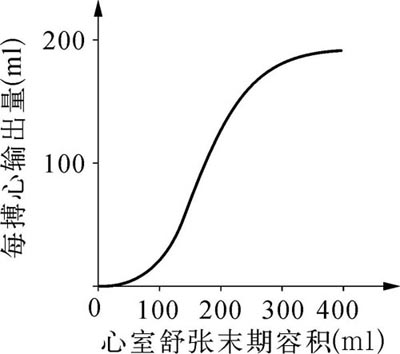
\includegraphics{./images/Image00028.jpg}
 \captionsetup{justification=centering}
 \caption{Starling曲线}
 \label{fig4-1}
  \end{figure} 

\subsubsection{什么是心功能曲线,有何临床意义?}

心功能曲线反映心室前负荷与心室每搏做功之间的关系。临床上常以压力指标反映前负荷。以左心室舒张末期压力为横轴、左室每搏功为纵轴做图,可以得到两者相互关系的曲线(图\ref{fig4-2}),称为心功能曲线(ventricular
function curve)。

\protect\hypertarget{text00010.htmlux5cux23ck001}{}{}
\begin{figure}[!htbp]
 \centering
 
\includegraphics{./images/Image00029.jpg}
 \captionsetup{justification=centering}
 \caption{心功能曲线}
 \label{fig4-2}
  \end{figure} 

心功能曲线大致可以分为3段:①心室充盈压在12~15mmHg的范围内(相当于16~20cm
H\textsubscript{2}
O),是心室的最适前负荷。一般情况下左心室充盈压为5~6mmHg,处于心功能曲线左侧的升支段,和最适前负荷还有一段距离。因而,心室每搏做功随心室充盈压的增加而增加,说明心室肌有较大的初长度储备。这种通过心肌细胞本身初长度的改变而引起心肌收缩强度的变化,称为异长自身调节,它保证了心输出量能随回心血量的增加而增加,使心室舒张末期容积和压力维持在正常范围之内,同时在左、右心室保持基本相同心输出量中也具有重要的调节作用。②心室充盈压在15~20mmHg(相当于20~27cm
H\textsubscript{2}
O)的范围内,曲线趋于平坦,说明通过心室肌初长度变化调节其收缩功能的作用较小。③心室充盈压进一步升高(>20mmHg),曲线平坦或轻度下倾,但并不出现降支。只有当心室出现严重的病理变化时,心室每搏做功才会随心室充盈压进一步增加而下降。

\subsubsection{什么是心室顺应性曲线?}

心室等容舒张期末,左心室内压力下降至低于左心房压力时,二尖瓣开放,左心室开始充盈。随着左心室被逐渐充盈,心室内容积逐渐增加,压力也有所增加,心室舒张期的压力与容积的变化不是直线关系,这条曲线实际上代表了左心室的顺应性(图\ref{fig4-3})。当心脏顺应性下降时,心室顺应性曲线向左上方移位,见于心肌缺血、心肌肥厚、限制性心肌病、左右心室失协调、心包填塞及感染性休克早期;反之,当心室顺应性增加时,曲线向右上方移位,见于感染性休克中后期、扩张型心肌病以及心包填塞解决后。在心室顺应性降低的情况下,改善心肌顺应性对于维持心脏功能十分重要,积极治疗原发病有助于改善心肌顺应性,此外,硝酸酯类药物和米力农类药物也可改善心室顺应性。

\begin{figure}[!htbp]
 \centering
 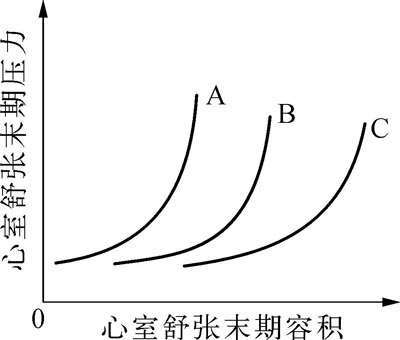
\includegraphics{./images/Image00030.jpg}
 \captionsetup{justification=centering}
 \caption{心室顺应性曲线}
 \label{fig4-3}
  \end{figure} 

A.为心室顺应性降低;B.为心室顺应性正常;C.为心室顺应性增高。

\subsubsection{怎样进行动脉血压监测,如何分析动脉波形?}

动脉血压监测可分为有创和无创监测两种。无创是指通过传统的袖带听诊、振荡控制描记器来进行血压监测,简单易行,临床多采用,但对于重症患者不够准确;有创是指通过动脉置管直接监测动脉血压,对于休克等重症患者,推荐采用动脉置管直接测压,可以准确及时反映动脉血压。

正常动脉压力波分为升支、降支和重搏波(图\ref{fig4-4}),升支表示心室快速射血进入主动脉,至顶峰为收缩压,正常值为100~140mmHg(1mmHg=0.133kPa);降支表示血液经大动脉流向外周,当心室内压力低于主动脉时,主动脉瓣关闭与大动脉弹性回缩同时形成重搏波。之后动脉内压力继续下降至最低点,为舒张压,正常值60~90mmHg。从主动脉到周围动脉,随着动脉管径和血管弹性的降低,动脉压力波形也随之变化,表现为升支逐渐陡峭,波幅逐渐增加,因此股动脉的收缩压要比主动脉高,下肢动脉的收缩压比上肢高,舒张压所受的影响较小,不同部位的平均动脉压比较接近。测量位置距离主动脉越远,压力会越高;测量位置距离主动脉越远,波形中重搏切迹越不明显。

\begin{figure}[!htbp]
 \centering
 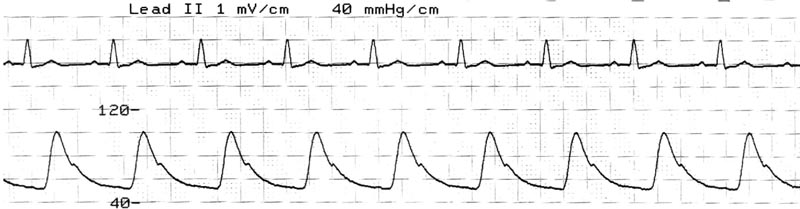
\includegraphics{./images/Image00031.jpg}
 \captionsetup{justification=centering}
 \caption{正常动脉压波形}
 \label{fig4-4}
  \end{figure} 

\subsubsection{有创动脉监测的途径应怎么选择?}

周围动脉置管位置选择总的原则是:局部侧支循环丰富,即使发生局部动脉阻塞亦不会引起远端组织缺血性损伤。一般可选择桡动脉、肱动脉、股动脉和足背动脉等。由于桡动脉与尺动脉之间有动脉环,故临床上多选择桡动脉(常采用左侧,左手功能占优势者采用右手)。位于腕部桡侧腕屈肌腱的外侧可清楚摸到其搏动,由于位置表浅且相对固定,穿刺置管较易成功,它与尺动脉在掌部组成掌深、浅动脉弓(侧支循环丰富),即使桡动脉发生阻塞或栓塞也不会影响手部的血供。

桡动脉穿刺前必须测试尺动脉血流是否通畅,可用改良式Allen试验法测试,具体方法:①测试者以手指压迫患者桡动脉以阻断桡动脉血流,让病人将手举过头顶并连做握拳动作数次,然后紧紧握拳;②测试者继续压迫桡动脉让患者将手下垂,并自然伸开手掌;③观察手掌部颜色由白转红的时间,若尺动脉畅通和掌弓循环良好,转红的时间多在3秒左右,在6秒钟以内转红,提示Allen试验阴性,若在7~15秒钟转红,说明尺动脉血供延迟,称为Allen试验可疑,如果15秒以上仍不转红则说明尺动脉血供有障碍,即Allen试验阳性,此时桡动脉不宜采用。

\subsubsection{动脉穿刺置管有哪些并发症,怎样防治?}

动脉穿刺置管常见的并发症有血栓形成、动脉栓塞、出血和感染等。

周围动脉穿刺置管引起血栓形成的因素是多方面的------①血栓形成与套管留置时间呈正比:套管留置时间越长,血栓发生率越高,如18号套管桡动脉置管20小时血栓发生率为25%,20~40小时血栓形成的发生率高达50%;②血栓形成与套管内径和血管内径大小密切相关:套管内径与动脉内径的比值越大发生率越高,用20号套管比18号套管进行动脉穿刺置管,血栓发生率明显减少。股动脉或肱动脉置管血栓发生率明显低于桡动脉置管;③血栓形成与套管针材料有关:同样型号套管留置时间相同,聚乙烯套管血栓形成的发生率为90%,而聚四氟乙烯套管仅为29%;④血栓形成与穿刺次数有关:多次反复穿刺造成血管内膜的损伤可增加血栓发生率。

动脉栓塞的栓子多来自测压管道和套管针内形成的血凝块。持续冲洗装置可减少栓塞的机会,而间断冲洗时间不易掌握,动脉栓塞易于发生。

穿刺损伤常引起局部出血和血肿形成,穿刺成功置管后局部加压止血3~5分钟。在行股动脉穿刺时当进针位置过高时可误伤髂外动脉而造成腹膜后出血,如不及时发现,后果十分严重。当术后拔除测压套管时应局部加压30分钟。

感染多由于置管时间太长引起,一般保留3~4天应拔除测压套管。如术后发现局部有炎症表现应及时拔除,若病情需要应改换部位重新穿刺。

\subsubsection{什么是中心静脉压,有何临床意义?}

中心静脉压是通过中心静脉置管测得的胸腔内大血管或右心房内的压力,是反映有效循环血容量的压力指标。当患者无三尖瓣病变时,中心静脉压可以反映右心室舒张末压力,间接评价右心室前负荷。

1962年Wilson首先开展的床边中心静脉压监测,是床旁有创血流动力学监测的开端。

\subsubsection{中心静脉穿刺置管途径有哪些?穿刺应注意哪些问题?}

目前多采用经皮穿刺的方法放置导管至中心静脉,常用的穿刺部位有颈内静脉、锁骨下静脉或股静脉。

中心静脉穿刺时的注意事项:

(1)应掌握多种径路的穿刺技术,不可强调因某一径路的穿刺成功率高而进行反复多次的穿刺,否则会造成局部组织的严重创伤和血肿。

(2)严重的低血容量状态时,由于静脉血管容量不足,静脉壁塌瘪,有时穿透静脉也未能抽得回血,这时需缓慢退针,边退针边抽吸,往往在退针过程中抽得静脉回血。

(3)在严重的低血容量状态时,由于正式穿刺用粗针头相对较钝,可将静脉壁向前推移甚至压瘪,所以正式穿刺时的进针深度往往较试穿时要深。

(4)穿刺过程中,穿刺针要直进和直退,若需改变穿刺方向时必须将针尖退至皮下,否则增加血管的损伤。

(5)穿刺成功后,应迅速将导管内气体抽出注入肝素生理盐水,以防在固定导管时血液在管内凝固。

(6)在固定导管时,缝针的方向一定与导管的走向平行,切不可横跨导管,以免在皮下穿破导管。

\subsubsection{Swan-Ganz肺动脉漂浮导管血流动力学监测的适应证和禁忌证有哪些?}

Swan-Ganz肺动脉漂浮导管血流动力学监测,是临床上最常用的有创性血流动力学监测手段之一,肺动脉漂浮导管适用于对血流动力学指标、肺脏和机体组织氧合功能的监测,任何原因引起的血流动力学不稳定及氧合功能改变,或存在可能引起这些改变的危险因素,均为血流动力学监测的适应证。该检测的意义概括起来主要有两个方面(表\ref{tab4-1}):第一,明确诊断;第二,指导治疗、判断疗效。

\begin{table}[htbp]
\centering
\caption{血流动力学监测的临床应用}
\label{tab4-1}
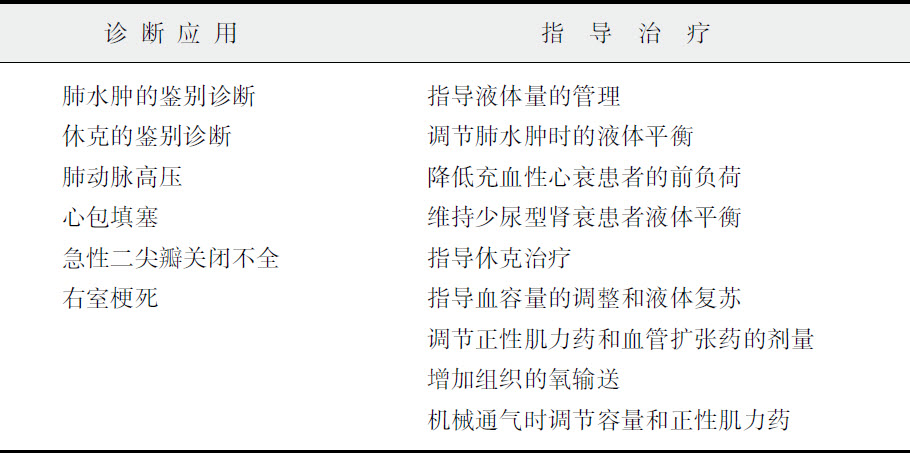
\includegraphics{./images/Image00032.jpg}
\end{table}

血流动力学监测无绝对禁忌证,但对于下列情况应谨慎使用:①肝素过敏;②穿刺局部疑有感染或已有感染;③严重出血性疾病或溶栓和应用大剂量肝素抗凝;④完全性左束支传导阻滞(置入肺动脉漂浮导管的过程中可能伤及右束支,引起完全性房室传导阻滞,心跳骤停);⑤心脏及大血管内有附壁血栓。

\subsubsection{如何在压力波形指导下放置Swan-Ganz肺动脉漂浮导管?}

接受血流动力学监测的患者大多数病情危重,不宜搬动。放置Swan-Ganz肺动脉漂浮导管只能在床边进行,只能根据压力波形指导放置Swan-Ganz肺动脉漂浮导管。

常用的Swan-Ganz肺动脉漂浮导管的置管途径有颈内静脉及锁骨下静脉。临床应根据术者的经验和习惯、患者的解剖特点及特殊临床情况,综合考虑来选择穿刺部位。右侧颈内静脉常作为肺动脉漂浮导管首选置管途径。应用Seldinger导丝法穿刺置管,将导管的自然曲度朝向右心室流出道,便于导管顺利进入右心室和肺动脉。其过程如下:

(1)导管进入右心房 导管顶端进入右房后,压力显示典型的心房压力波形,表现为a、c、v波,压力波动的幅度很小(图\ref{fig4-6})。此时气囊应充气1~1.5ml,锁住三通,继续向前送入导管。

(2)导管进入右心室 一旦导管顶端通过三尖瓣,压力波形突然改变,收缩压明显升高至25mmHg左右,舒张压不变或略有下降,脉压明显增大,压力曲线的上升支带有顿挫,这种波形提示导管尖端进入右心室(图\ref{fig4-5})。

导管在右室内、尤其是进入右心室流出道时,可刺激心室壁引起室性早搏、甚至室颤。确保气囊充盈、减少右室停留时间,可减少心律失常的发生。操作过程中也可将患者头抬高5°,右侧倾斜卧位,可减少导管对心脏的刺激。

(3)导管进入肺动脉 导管尖端进入右心室后,应迅速而轻柔地送入导管,当收缩压基本保持不变、舒张压明显升高、平均压升高、压力曲线的下降支出现重搏波切迹时,表明导管已进入肺动脉。

(4)肺动脉嵌顿 继续送入导管,导管气囊嵌顿时,收缩压舒张压下降,脉压差明显减小,平均压力低于肺动脉平均压。如无波形干扰,可分辨出a、c、v波。这时,应停止移动导管,立即排空气囊,可见压力波形马上转为肺动脉压力波形。再次充盈和排空气囊,压力波形重复出现肺动脉嵌顿压力波形和肺动脉压力波形,说明导管位置良好(图\ref{fig4-5})。

\begin{figure}[!htbp]
 \centering
 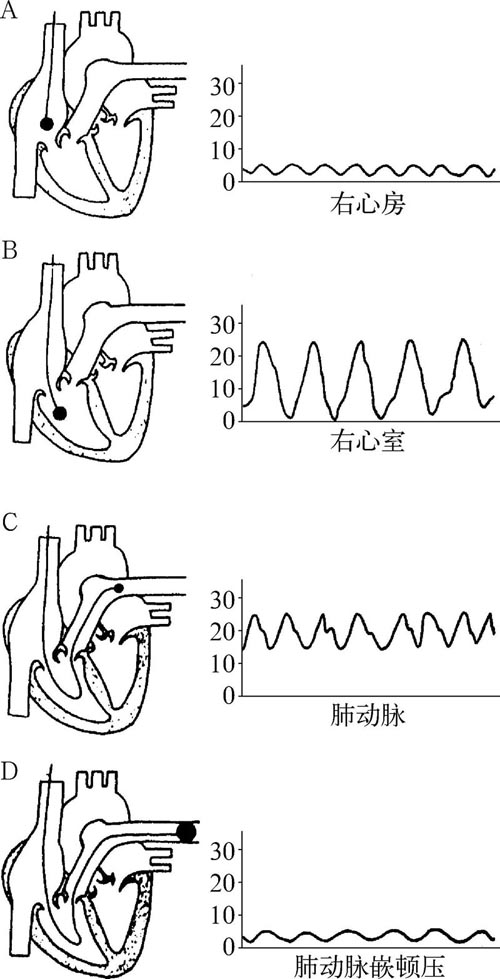
\includegraphics{./images/Image00033.jpg}
 \captionsetup{justification=centering}
 \caption{肺动脉漂浮导管在右房、右室、肺动脉及嵌顿不同部位的压力波形}
 \label{fig4-5}
  \end{figure} 

导管顶端从右室到嵌顿位的深度一般10~15cm。右颈内静脉到嵌顿部位的距离为40~50cm。若导管入右室再继续前行距离超过15cm仍不能嵌顿,应排空气囊把导管退回至右房后再重新插入,因为导管在心腔内过长易打结。

若气囊充气量<1.0ml时即出现嵌顿波,说明导管置入过深,应退出。每次充盈时都应注意嵌顿所需最小气囊容量。导管向远端移位、气囊过分充盈、气囊偏心及导管嵌顿时冲洗导管易引起肺动脉破裂。

\subsubsection{如何判断心房波的各波形?}

在窦性心律时,心房压力波的特征为两个大的正向波(a和v波)、两个负向波(X和Y降波)和另外一个小的正向波c波(图\ref{fig4-6})。a波由心房收缩产生。随后为心房舒张和心室收缩带动三尖瓣环关闭,房室连接处向下运动产生负向X波。三尖瓣关闭时瓣叶轻度向右房突出引起右房压轻微增加形成c波,可呈明显的波形或作为a波的挫折,有时不出现。X降波后的正向波为v波,为心室收缩时心房被动充盈产生。最后的一个波为Y降波,标志着三尖瓣开放,右房快速排空血液进入右心室。

\begin{figure}[!htbp]
 \centering
 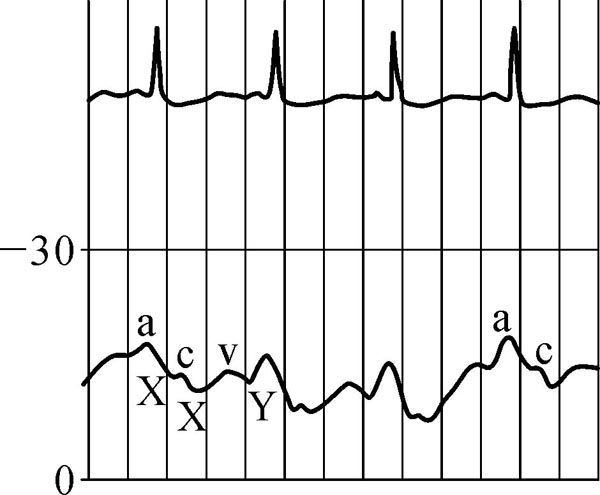
\includegraphics{./images/Image00034.jpg}
 \captionsetup{justification=centering}
 \caption{心房压力波}
 \label{fig4-6}
  \end{figure} 

\subsubsection{如何判断Swan-Ganz肺动脉导管顶端位于肺的Ⅲ区?}

20世纪60年代,West根据人体站立位时肺泡内压力和肺血管压力的关系,将肺组织分为3区(图\ref{fig4-7})。正常人Ⅰ区指肺泡内压高于肺动脉、肺静脉压,肺毛细血管通常处于关闭状态,肺血管内几乎无血流;Ⅱ区是肺泡内压力于吸气相低于肺动脉压和肺静脉压,呼气相高于肺静脉但低于肺动脉压,血流取决于肺动脉和肺泡间的平衡,一旦Swan-Ganz肺动脉导管气囊充盈阻断血流,即可由Ⅱ区变为Ⅰ区;Ⅲ区肺泡内压始终低于肺血管内压力,肺毛细血管始终保持开放,形成肺动脉与左房之间的自由通道。因Ⅰ区、Ⅱ区肺血管内持续或间断无血流,所测定的肺动脉嵌顿压只能反映肺泡内压力,并不反映左房压。因此,只有Ⅲ区肺血管内有持续血流,测定的肺动脉嵌顿压可反映左房压及左室舒张末压。

\begin{figure}[!htbp]
 \centering
 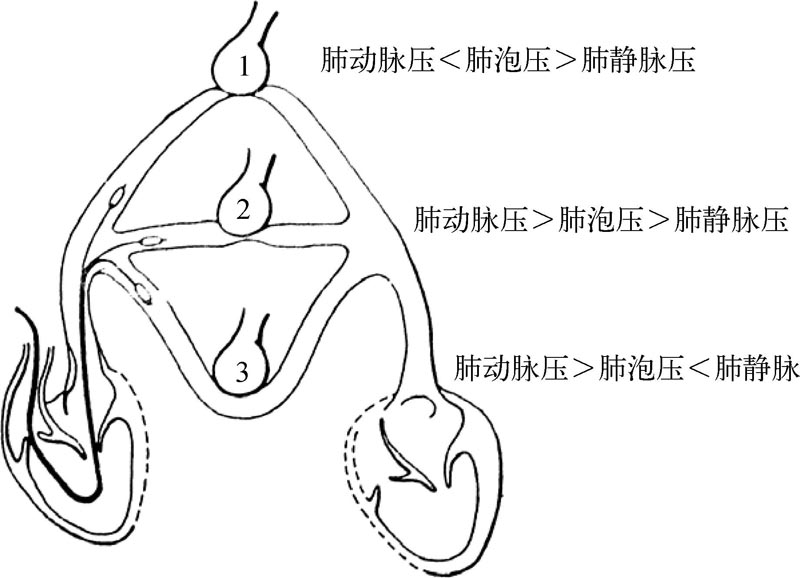
\includegraphics{./images/Image00035.jpg}
 \captionsetup{justification=centering}
 \caption{West肺区模型}
 \label{fig4-7}
  \end{figure} 

确定导管顶端位于Ⅲ区有以下几项指标:①具有典型肺动脉压和肺动脉嵌顿压波形;②肺动脉舒张压大于肺动脉嵌顿压;③呼气末正压试验------突然撤离呼气末正压,肺动脉嵌顿压的改变小于呼气末正压改变的一半。

\subsubsection{放置Swan-Ganz肺动脉漂浮导管的可能并发症及防治措施有哪些?}

血流动力学监测的并发症与插管过程及导管留置有关(表\ref{tab4-2}),但致命性的严重并发症发生率并不高。遵循操作常规,严守无菌原则,可最大限度地避免并发症的发生。

\begin{table}[htbp]
\centering
\caption{肺动脉漂浮导管相关的并发症}
\label{tab4-2}
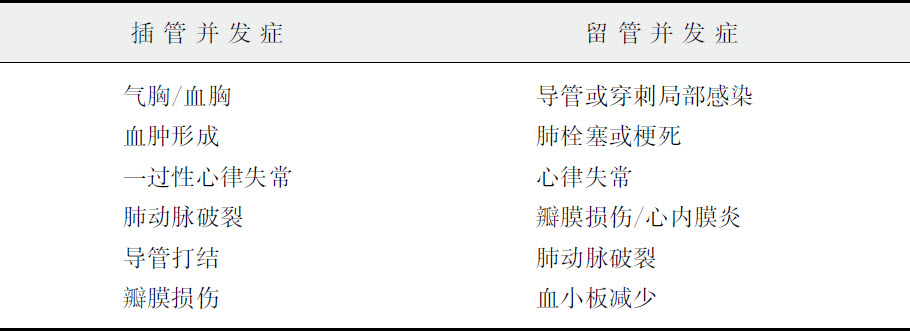
\includegraphics{./images/Image00036.jpg}
\end{table}

(1)心律失常 插管和导管留置过程中均可发生心律失常。室性早搏和一过性室性心动过速最为常见,主要由导管顶端刺激心室壁所致。室性心律失常的发生率在11%~68%。导管通过右心室时发生的室性心动过速,通常只要导管顶端通过肺动脉瓣即自动终止,因此无需处理。仅1.3%~1.5%的导管相关室性心动过速需抗心律失常药物、心前区捶击或电复律治疗。持续而不能自行转复的室性心动过速和室颤的发生率极低,不推荐预防性应用利多卡因。在急性心肌梗死或其他心律失常高危的患者,在插入肺动脉漂浮导管时,应预先准备好相应的治疗和抢救设备。

右束支传导阻滞的发生率为0.05%~5%,而且多为一过性的。但如果患者存在完全性左束支传导阻滞,即使一过性的右束支传导阻滞也可导致心跳骤停的严重后果。左束支传导阻滞的患者放置肺动脉漂浮导管前,不必常规放置临时起搏器,可选用带有起搏功能的改良型肺动脉漂浮导管,或在床边备一体外起搏器,以备发生完全性房室传导阻滞或心跳骤停时所需。

导管相关的心律失常多与导管的机械刺激有关,在插管和导管留置时采取以下措施,可有效预防或减少心律失常的发生:①心肌缺血、休克、低氧血症、电解质紊乱、酸中毒和(或)高内源性儿茶酚胺水平的患者发生室性心律失常的几率高,术前应尽量纠正;②导管到达右心房后,应立即充盈气囊,以减少导管顶端对心内膜的刺激;③导管通过三尖瓣进入右心室后,应快速轻柔地送入导管,使导管向上反折经右心室流出道进入肺动脉,尽量缩短导管在右心室内停留时间。

(2)血栓形成及栓塞 大多数经颈内静脉放置过肺动脉漂浮导管的患者,静脉造影或尸检发现在穿刺部位有血栓形成,通常没有临床表现。血栓也可发生在心脏内或肺动脉中,但发生率极低。导管本身可阻塞血管而引起肺梗死,通常与导管放置过深有关,使得肺动脉在气囊排空时仍处于部分嵌顿状态。梗死范围较小时通常无临床表现,仅在导管顶端外侧有新的肺部阴影。

预防措施:①使用肝素生理盐水持续冲洗导管或选用肝素包被的导管;②测肺动脉嵌顿压的时间不宜过长,一般不超过2~3个呼吸周期;③气囊放气排空后压力波形应为肺动脉压力波形,如持续为嵌压波形,提示导管过深,应缓慢向外退导管,直至出现肺动脉压力波形;④放置导管后,应常规做X线胸部检查,确定导管位置。

(3)肺动脉破裂 肺动脉破裂是Swan-Ganz肺动脉漂浮导管血流动力学监测中最严重的并发症。典型表现为突然大咯血,病死率接近50%,但发生率仅0.06%~0.2%,多见于高龄、肺动脉高压、低温体外循环心脏手术以及其他抗凝治疗的患者。最主要的原因是导管位置过深或气囊偏心等。若此时充盈气囊或快速注射液体,易造成肺动脉破裂。因此,避免导管向远端移位和气囊过度充盈,可以降低肺动脉破裂的危险性。

肺动脉破裂的防治:①气囊未充盈时,禁止向前推送导管;②测肺动脉嵌顿压时,应缓慢充盈气囊,当肺动脉压波形变为肺动脉嵌顿压波形时,应立即停止继续充气;③禁止用液体充盈气囊;④尽量减少气囊充盈、导管嵌顿时间,减少气囊充盈次数。如果肺动脉舒张压与肺动脉嵌顿压有良好的相关性,则可用肺动脉舒张压估计肺动脉嵌顿压;⑤导管不可置入过深;⑥一旦发生大咯血,应保持气道通畅,立即建立人工气道、气管插管,首选双腔气管插管,必要时进行手术治疗。

(4)导管打结 常见原因是导管在右心室或右心房内缠绕,易发生在扩大的右心房或右心室。如果自心房或心室向前推送导管15cm以上仍无压力改变,需考虑导管打圈或缠绕,应放掉气囊、缓慢撤回导管。导管退回后,可用冰生理盐水冲洗导管,增加导管硬度后再送入。插管过程中,应避免一次将导管送入过长。调整导管位置时遇到阻力,应首先想到导管打结,切勿用强力将导管退出。

如高度怀疑导管打结,应立即在X线下证实,并置入导引钢丝,松解导管结后将其退出体外。如果导管结无法松解或其中含有腱索、乳头肌等心内结构,则需采取外科手术取出导管。

(5)感染 导管留置期间,穿刺局部出现红、肿、痛、皮温升高,或出现发热、寒战,应考虑肺动脉漂浮导管相关感染,应立即将导管拔出,同时取穿刺局部分泌物、导管血和外周静脉血、导管远端送培养,并做抗菌药物敏感试验。必要时给予抗感染治疗。

预防措施:①在所有与导管相关的操作中,严格遵循无菌原则;②插管局部每天常规消毒,更换敷料,敷料被浸湿或污染时随时更换;③尽量减少测定心输出量及抽取混合静脉血的次数;④尽量缩短肺动脉漂浮导管的留置时间。研究表明,导管留置时间超过72小时,导管相关感染的发生率明显增加。

\subsubsection{Swan-Ganz肺动脉漂浮导管准确的压力监测应重点注意什么?}

压力监测系统包括:①导管和测压连接管;②压力传感器;③冲洗装置;④压力监测仪。进行压力监测时应注意:

(1)压力传感器的连接 压力传感器一端与压力监测仪连接,另一端直接或经测压连接管连于肺动脉漂浮导管的顶端开口,以保证在插管过程中持续监测导管顶端的压力。根据压力波形及数值的变化确定导管位置。另一个压力传感器连接于肺动脉漂浮导管的近端开口,监测右房压。

(2)监护仪的设置 监护仪应置于操作者可见处。压力尺度根据患者的具体情况设定,一般患者设为0~50mmHg。

(3)参照点的选择及调零 所有测量的压力都是相对于大气压的,换能器的气液面应以右心房水平作为参照点调零。临床通常将腋中线第4肋间水平作为确定仰卧位患者参照点的标志。将压力传感器置于参照点水平,通向大气调零。在压力监测过程中,若改变压力传感器放置水平将使所测压力值高于或低于实际压力。

(4)测压系统的阻尼检测 导管插入前应先做快速冲洗试验,以证实整个测压系统阻尼正常(图\ref{fig4-8})。挤压换能器的冲洗器快速冲洗1秒,然后松开。阻尼正常时,压力迅速上升呈一方波,然后陡直下降超过基线,称为过射(overshoot),又迅速回复至基线水平。阻尼过大时压力下降缓慢,逐渐回至基线水平,而无过射现象。阻尼不足时有过射波出现,但过射的压力波不能迅速回复至基线水平。阻尼过大多与测压系统内存在气泡有关,气泡的顺应性远大于液体的顺应性,可造成很强的压力返折。阻尼不足主要由连接处松开或连接管不正确引起。插管后阻尼过度的原因还包括管腔内有回血,导管顶端有血块,导管顶端贴壁及三通未完全打开等。

\begin{figure}[!htbp]
 \centering
 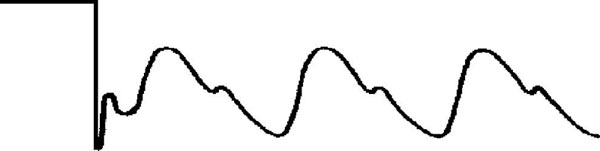
\includegraphics{./images/Image00037.jpg}
 \captionsetup{justification=centering}
 \caption{测压系统阻尼的快速冲洗试验}
 \label{fig4-8}
  \end{figure} 

\subsubsection{Swan-Ganz肺动脉漂浮导管能获得哪些血流动力学指标?}

可以直接获得部分血流动力学指标,并通过计算间接获得其他指标。血流动力学监测的目的是通过分析心血管系统不同部位的压力、流量及阻力之间的相互关系,对心脏的前负荷、后负荷及心脏的收缩舒张功能做出判断,指导临床诊断与治疗。

通过Swan-Ganz肺动脉漂浮导管进行血流动力学监测,部分指标可通过直接测量得到,部分根据公式计算而来(表\ref{tab4-3})。\footnote{*MAP:平均动脉压力;PAP:肺动脉压力;CVP:中心静脉压力;PAWP:肺动脉嵌顿压力。}

\begin{table}[htbp]
\centering
\caption{血流动力学监测指标及参考正常范围\textsuperscript{*}}
\label{tab4-3}
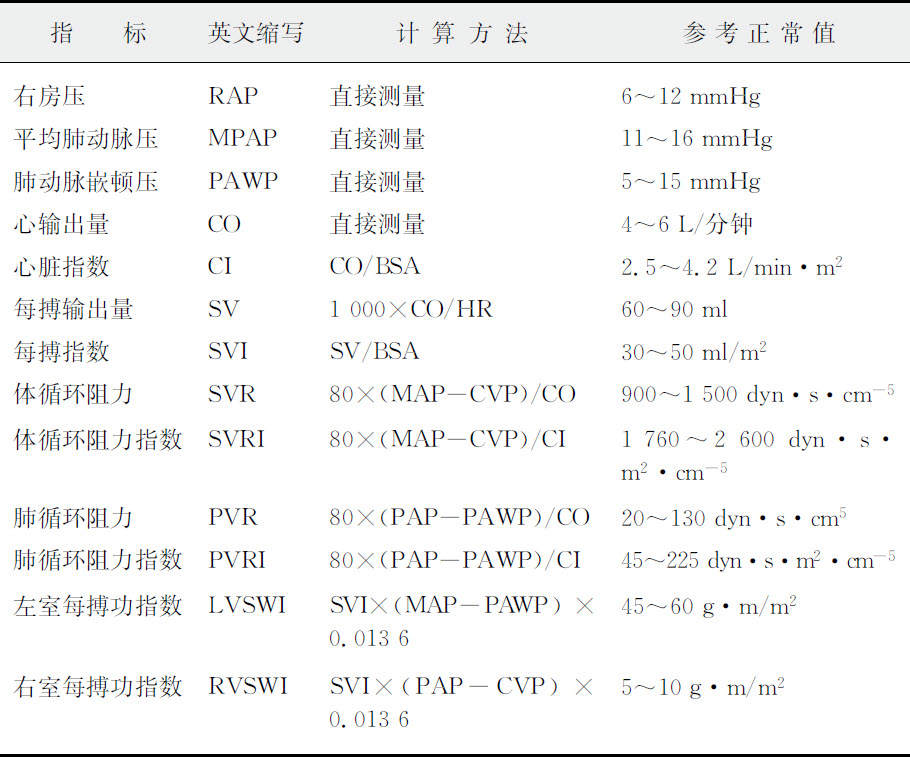
\includegraphics{./images/Image00038.jpg}
\end{table}

\subsubsection{中心静脉压和肺动脉嵌顿压能反映心脏前负荷吗?}

中心静脉压反映右心室舒张末压,肺动脉嵌顿压则反映左心室舒张末压,都是反映前负荷的压力指标。

中心静脉压和肺动脉嵌顿压的临床价值存在争议。有研究表明,中心静脉压不能反映心脏前负荷情况。即使是在健康志愿者中,中心静脉压和肺动脉嵌顿压也与心室的充盈程度没有必然的关联。此外,除去医务人员的技术原因,还有其他因素影响中心静脉压与肺动脉嵌顿压测定,如心率、心室顺应性、肺静脉压、胸腔内压等。正压通气和低于10mmHg的呼气末正压一般不会影响肺动脉嵌顿压,而高于10mmHg的呼气末正压则会使肺动脉嵌顿压测量值明显升高。动物实验表明,腹腔高压或腹腔室间隔综合征可提高中心静脉压和肺动脉嵌顿压,腹内压达到20mmHg以上时尤其显著。因此,中心静脉压和肺动脉嵌顿压在一定程度上反映心脏前负荷,但绝对测量值往往不能准确反映心脏前负荷,在参考基线水平的基础上观察其动态变化有一定临床意义。

\subsubsection{如何动态监测中心静脉压和肺动脉嵌顿压来间接反映心脏前负荷?}

中心静脉压是反映患者血容量状态的指标之一。正常值为5~10cm
H\textsubscript{2} O(1cm H\textsubscript{2}
O=0.098kPa)。中心静脉压<5cm H\textsubscript{2}
O提示血容量不足;中心静脉压>15cm H\textsubscript{2}
O提示输液过多或心功能不全。

连续、动态监测中心静脉压的改变具有重要临床意义。通过容量负荷试验观察中心静脉压的改变,可判断患者的容量情况,对治疗具有重要价值。容量负荷试验的具体步骤包括:①测定并记录中心静脉压基础水平;②根据患者情况,10分钟内快速静脉滴注生理盐水50~200ml;③观察患者症状、体征的改变;④观察中心静脉压改变的幅度(2~5cm
H\textsubscript{2} O原则)(表\ref{tab4-4})。

\begin{table}[htbp]
\centering
\caption{中心静脉压(CVP)导向的容量负荷试验}
\label{tab4-4}
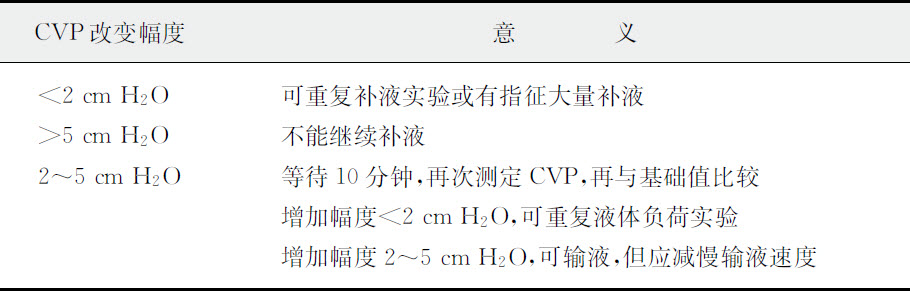
\includegraphics{./images/Image00039.jpg}
\end{table}

肺动脉嵌顿压可通过肺动脉漂浮导管监测。肺动脉嵌顿压是反映左心室前负荷水平的指标。与中心静脉压相比,能够更准确地反映机体容量状态。正常值为8~15mmHg。肺动脉嵌顿压<6mmHg提示容量严重不足;肺动脉嵌顿压<12mmHg仍提示容量不足;肺动脉嵌顿压12~15mmHg提示容量正常或容量不足伴左心功能不全;肺动脉嵌顿压>15mmHg提示容量过多或伴左心功能不全,有发生肺水肿的危险性。

通过容量负荷试验,观察肺动脉嵌顿压的改变可判断患者的容量情况,对治疗具有重要价值。容量负荷试验的具体步骤包括:①观察患者症状、体征(心率、血压、尿量、四肢温度、意识状态、肺部湿啰音及哮鸣音),测定并记录肺动脉嵌顿压的基础水平;②根据患者情况,10分钟内快速静脉滴注生理盐水50~200ml;③观察患者症状、生命体征的改变;④观察肺动脉嵌顿压改变的幅度(3~7mmHg原则)(表\ref{tab4-5})。

\begin{table}[htbp]
\centering
\caption{肺动脉嵌顿压导向的容量负荷试验}
\label{tab4-5}
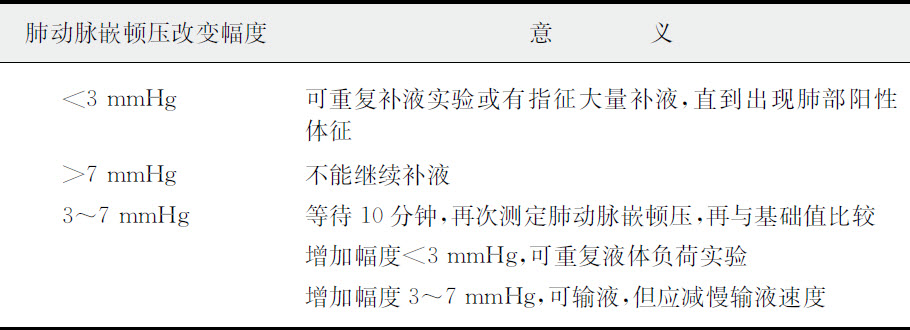
\includegraphics{./images/Image00040.jpg}
\end{table}

\subsubsection{呼吸运动对压力监测有什么影响?如何避免?}

在呼吸周期内,胸膜腔内的压力变化会导致动脉内或心腔内压力的变化,从而影响压力监测。自主呼吸时,吸气时胸腔内压力下降,呼气时压力上升,中心静脉压和肺动脉嵌顿压的波形会受到干扰,影响测定结果;机械通气时,情况相反(图\ref{fig4-9})。因此,在呼气末进行压力测量(胸膜腔压力接近零点),可以将呼吸对压力监测的影响最小化。

\begin{figure}[!htbp]
 \centering
 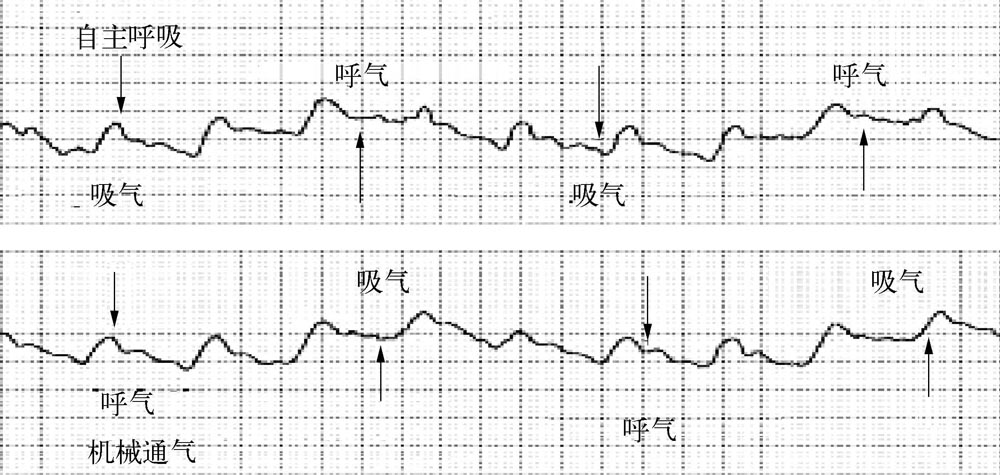
\includegraphics{./images/Image00041.jpg}
 \captionsetup{justification=centering}
 \caption{呼吸对压力波形的影响}
 \label{fig4-9}
  \end{figure} 

\subsubsection{如何测定肺动脉嵌顿压?}

肺动脉嵌顿压是通过向Swan-Ganz肺动脉漂浮导管气囊注射1.0~1.5ml空气,使导管顶端在肺动脉分支内前行直至阻塞前向血流而测得的。由于肺循环是低压系统,而且没有静脉瓣,因此,理论上肺动脉嵌顿压与左心室舒张末期压力有相关性。要保持这种相关性,必须保证压力传导通路通畅,导管确实嵌顿以及足够的平衡时间。平衡时间指心脏搏动的舒张期。研究显示,心率在130次/分以上时,由于舒张期明显缩短,可以导致肺动脉嵌顿压的测定值升高。

临床上把肺动脉嵌顿压作为评估肺毛细血管静水压和左心室前负荷的一项重要指标,但肺动脉嵌顿压并不等同于肺毛细血管压,也不是反映左心前负荷的直接指标。

\subsubsection{Swan-Ganz肺动脉漂浮导管测定心输出量的原理是什么?}

Swan-Ganz肺动脉漂浮导管利用热稀释法来测量心输出量。热稀释法的基本原理是从肺动脉漂浮导管右房开口快速均匀地注入低于血温的液体,注入的液体混入血液使血温发生变化,血液经右房、右室达肺动脉,导管远端的热敏电阻感知注射低温液体后血液温度变化,心输出量计算仪描绘并处理温度变化曲线,按Stewart-Hamilton公式计算出心输出量。

热稀释曲线最高点为最低温度点,即与基础血温差别最大的点。心输出量大、血流较快、液体注入后血温变化小,曲线下面积小;心输出量较低、血流缓慢、曲线下面积大。因此,心输出量数值与曲线下的面积成反比(图\ref{fig4-10})。

\begin{figure}[!htbp]
 \centering
 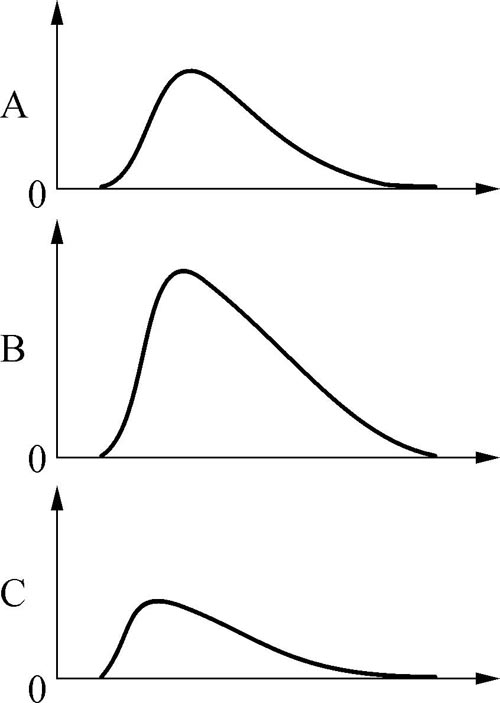
\includegraphics{./images/Image00042.jpg}
 \captionsetup{justification=centering}
 \caption{测定心输出量的热稀释曲线}
 \label{fig4-10}
  \end{figure} 

A.正常心输出量(6L/分钟);B.低心输出量(3L/分钟);C.高心输出量(12L/分钟)

热稀释曲线上升支反映推注速度。推注速度越慢,上升支越平缓;推注速度越快,上升支越陡直。热稀释曲线下降支及曲线下面积与右心血流量相关,慢而长的降支使曲线下面积增大,表明血流量小,心输出量低;相反,降支快、面积小,表明血流量大,温度变化较快,心输出量高。

\subsubsection{热稀释法测量心输出量的影响因素及处理原则是什么?}

稀释法测量心输出量受多种因素影响,为了使测量结果更准确,在测量过程中应注意以下问题。

(1)注射液体的温度 一般要求注射液体与血液的温差在10℃以上,所以冰水或室温液体通常可作为心输出量测定时的注射液体,但当患者体温过低或环境温度过高时,均不宜用室温下的液体来测定心输出量。

测量注射液体温度的方法------①冰浴法(Bath):热敏电阻置于冰水混合物中,从容器中抽出冰水,应在30秒内进行测量,操作者避免将整个注射器握于手中。上述任一环节出问题,都可造成测量结果高于实际心输出量。②在线法(in-line):“T”形热敏电阻连在肺动脉漂浮导管的近端口,直接测量注射液体的温度,从而消除了前一种方法可能的误差,目前临床较为常用。

(2)注射液体的容量 注射液体容量必须与心输出量监测仪(监护仪)预设液体容积一致。如果注射液体有0.5ml的误差,测量结果可出现5%的误差。

(3)注射速度 应快速、匀速,以4秒为佳。注射速度过慢,热稀释曲线的上升支变得平缓,曲线下面积大,测量结果低于实际心输出量。

(4)两次测量的间隔时间 两次测量的间隔时间过短,会发生基线不稳或基线漂移。应当保证注射间隔时间,使肺动脉血液温度回升至基础水平。注射液温度为室温,须间隔35秒;注射液为冰水时注射间隔须延长至70秒以上。

(5)中心静脉快速大量输液 若在测量心输出量的同时从中心静脉大量快速输液,可使肺动脉处血温降低,造成热稀释曲线下面积变小的假象,导致所得心输出量结果高于实际值。

(6)呼吸、心率、体位和肢体活动 这些因素均可使热稀释曲线的基线波动,影响测量结果。尤其在呼吸周期中,肺动脉血温变化0.01~0.02℃,呼吸困难时变化更大,故应在呼吸周期的同一时期测量,一般选择在呼气末。

(7)三尖瓣反流及心内分流 三尖瓣反流时可使测量结果低于实际值,甚至测不出结果。存在左向右分流时,测量结果可能低于实际值。

\subsubsection{利用热稀释法可以连续测量心输出量吗?}

为了消除不同操作者注射技术不同和注射液温度的误差带来的影响,消除反复注射液体指示剂带来的容量负荷过高及心律失常,并达到实时监测的目的,由改良的肺动脉漂浮导管与一台特制的心输出量监测仪组成的持续心输出量监测系统,已于20世纪90年代初应用于临床。这种改良导管在右房开口远端相当于右心室部位,缠绕可产热的电阻丝作为热释放器,在安全范围内(<44℃),按双侧序列释放热能使局部的血液加温,血液流经右心室到达肺动脉时使相对“冷”的血液升温。肺动脉导管顶端的热敏电阻感受温度的变化,描绘出与注射冷液体时相似的热稀释曲线,计算出心输出量。每30~60秒仪器可自动显示前3~6分的平均心输出量,基本实现了心输出量的实时、动态监测。

热稀释法持续心输出量测定的准确性已得到公认,持续心输出量测定与传统的热稀释法高度相关。但是体温低于31℃或超过41℃时,持续心输出量监测均无法进行。

\subsubsection{如何评价Swan-Ganz肺动脉漂浮导管在重症医学科的应用?}

1970年,美国加州大学洛杉矶分校的Swan和Ganz医师首先将带气囊的肺动脉导管这一技术应用于临床。此后,用于血流动力学监测的肺动脉导管也常被称为漂浮导管或Swan-Ganz肺动脉漂浮导管。通过肺动脉导管可以获得大量血流动力学和氧输送相关信息,对危重患者的滴定式循环支持提供监测依据。由于肺动脉导管的临床可操作性较强,监测指标对临床处理的反应性好,使得这一技术在临床中迅速推广,成为血流动力学监测的“金标准”。但20世纪80年代后期开始,一些研究显示肺动脉导管并不改善病人预后,同时新的血流动力学监测手段不断出现,因此,临床应用肺动脉导管有了争议,但肺动脉导管目前仍然是血流动力学监测的重要手段。

肺动脉导管监测影响循环支持策略。几项荟萃分析显示,当组织氧合障碍发生之前即实施血流动力学监测,以血流动力学目标指导性治疗能够改善患者预后。而当已经出现组织氧合障碍,或已经导致多器官功能障碍综合征之后,血流动力学目标指导性治疗对患者预后影响小。2008年发布的重症感染和感染性休克治疗《指南》已不推荐将超高血流动力学目标无选择地应用于重症患者,仍然非常强调早期目标指导性治疗,在休克发生的初期(6小时内)将血流动力学调整至理想水平,有利于防止组织灌注不足和器官衰竭
\protect\hyperlink{text00010.htmlux5cux23ch6-9}{\textsuperscript{{[}6{]}}}
。

监测手段的准确应用和正确解读肺动脉导管测得数据是其合理指导临床治疗的前提。美国食品和药物管理局和美国心肺血液研究所的联合报告指出,只有在临床人员肺动脉导管应用水平得到长足提高后,才可能对肺动脉导管是否影响转归做出评估。美国食品和药品管理局在其针对肺动脉导管的备忘录中鼓励国际性多中心随机对照研究,并强烈建议进行严格的肺动脉导管临床培训,减少人员因素对研究结果的影响。有研究显示,即使得到了反映真实情况的肺动脉导管数据,仍然存在数据解读和临床处理失误的可能。欧美调查表明,有超过50%的临床医护人员不能正确理解肺动脉导管数据。

并发症对肺动脉导管血流动力学的监测也有明显影响。肺动脉导管是一项有创监测手段,在中心静脉穿刺、肺动脉导管的放置和持续监测过程中均可产生并发症,如穿刺部位血肿、气胸、血气胸、室上性心动过速、导管相关性感染等,多数情况下这些并发症并不严重,未直接导致患者病死率增高。严重并发症如室性心律失常、张力性气胸、急性心内膜炎和肺动脉栓塞破裂等的发生率极低(<0.5%),也不可能明显改变肺动脉导管监测人群的总体病死率。但是,应该强调对操作者进行严格培训,并尽量缩短监测时限,以减少并发症的发生。

总之,肺动脉导管目前仍然是危重病人血流动力学监测的重要手段,在应用过程中,必须选择合适的患者和合适的时机,同时不断提高医务人员肺动脉导管操作能力和应用能力,正确获取监测数据并正确解读,根据监测结果指导临床治疗,才有可能改善患者预后。

\subsubsection{什么是血流动力学的“ABC理论”?}

血流动力学的“ABC”理论(图\ref{fig4-11})是应用血流动力学监测对循环功能进行支持治疗的基础理论。

\begin{figure}[!htbp]
 \centering
 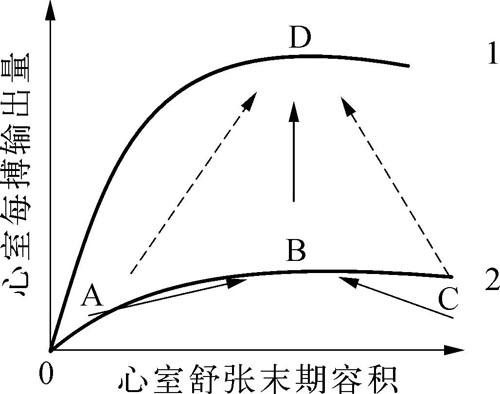
\includegraphics{./images/Image00043.jpg}
 \captionsetup{justification=centering}
 \caption{血流动力学“ABC”理论}
 \label{fig4-11}
  \end{figure} 

根据Starling定律,在正常情况下,随着心室舒张末期容积的增加,每搏输出量也相应增加。当心肌收缩力受损时,每搏输出量随舒张末容积增加而增长的程度明显下降,曲线呈低平状态。在进行临床血流动力学监测时,将每次测量的数据在图中标记出的点称为心功能点,D点则是治疗的目标点。如果初次测得患者的心功能点为A点,那么,应用心脏正性肌力药物和扩容治疗都可能使A点移向D点。如果首选应用心脏正性肌力药物,则曲线2移向曲线1,从而使A点沿虚线方向直接移向D点。如果首先进行扩容治疗,增加心脏的前负荷,若心功能正常,A点则沿曲线1移向D点,这是临床上所期望获得的结果。如果心肌功能受损,A点则沿曲线2移向B点。此时再应用正性肌力药物,心功能点则由B点移向D点。从A点不同的移动方向中可以看出,由A点到B点首先调整了心脏的前负荷,尽可能发挥了心脏自身的代偿作用,之后应用正性肌力药物使心功能点由B点移向D点,这时应用正性肌力药物的剂量明显少于由A点沿虚线移向D点所需的药物剂量,从而,正性肌力药物产生的副作用也明显减少。所以,A→B→D是将心功能点由A移向D的最佳选择。同理,如果患者的心功能点在C点,将心功能点由C移向D的最佳选择是C→B→D,而不应是由C点沿虚线直接到D点。

从这个示意图可以看出,心脏每搏输出量不足可能是由于心功能降低或同时并存前负荷过多或前负荷不足,调整心脏前负荷是获得最佳每搏输出量的首要治疗措施。只有在心脏自身处于最佳的做功状态后应用正性肌力药物才有可能取得最佳的治疗效果。对于心功能不全的患者一味地强调脱水或盲目地进行补液都同样带有片面性。

\subsection{氧代谢监测}

\subsubsection{如何计算氧输送和氧耗?}

氧输送(DO\textsubscript{2}
)指单位时间内由左心室向全身组织输送氧的总量,或者说是单位时间内动脉系统向全身输送氧的总量,其计算公式为:

\[
  \begin{array}{l}
DO_2=CI\times CaO_2\times 10\\
CaO_2  =Hb\times 1.34\times SaO_2+0.003\times PaO_2
  \end{array}
\]

从计算公式可知,氧输送取决于心脏指数(CI)、血红蛋白(Hb)含量和肺氧合功能[动脉血氧分压和动脉血氧饱和度(SaO\textsubscript{2}
)],因此氧输送直接受循环、血液及呼吸系统的影响。

氧耗(VO\textsubscript{2}
)指单位时间内组织细胞实际消耗氧的量,代表全身氧利用的情况,但并不能代表组织对氧的实际需要量(计算公式中混合静脉血氧含量反映经过组织代谢后循环血液中所剩余的氧。混合静脉血来自肺动脉):

\[
  \begin{array}{l}
VO_2=CI\times (CaO_2-CvO_2)\times 10\\
CvO_2  =Hb\times 1.34\times SvO_2+0.003\times PvO_2
  \end{array}
\]

\subsubsection{如何抽取混合静脉血?有何临床意义?}

混合静脉血是指从全身各组织回流并经过均匀混合后的静脉血。从肺动脉内取得的血是理想的混合静脉血标本。通过Swan-Ganz肺动脉漂浮导管可以获得混合静脉血标本。

抽取混合静脉血标本时,首先应确认Swan-Ganz肺动脉漂浮导管的顶端位于肺动脉内,压力波形显示典型的肺动脉波形。气囊予以排空,抽取混合静脉血标本速度要慢,否则可能抽取到氧合后血液,同时,在标本采集过程中,应隔绝空气,以免影响检测结果。

混合静脉血进行血气分析,可以反映全身氧代谢状况,指导重症患者的休克复苏。

\subsubsection{如何评价混合静脉血氧饱和度和中心静脉血氧饱和度的意义?}

混合静脉血氧饱和度反映组织器官摄取氧的状态。当全身氧输送降低或全身氧需求超过氧输送时,混和静脉血氧饱和度降低,提示机体无氧代谢增加。但当组织器官氧利用障碍或微血管分流增加时,可导致混和静脉血氧饱和度升高,尽管此时组织的氧需求量仍可能增加。

在休克早期,全身组织的灌注已经发生改变,即使血压、心率、尿量和中心静脉压仍处于正常范围,此时可能已出现混和静脉血氧饱和度降低,提示混和静脉血氧饱和度能较早发现病情的变化。

中心静脉血氧饱和度与混和静脉血氧饱和度有一定的相关性,在临床上更具可操作性,虽然测量的中心静脉血氧饱和度值要比混和静脉血氧饱和度值高5%~15%,但它们所代表的趋势是相同的,可以反映组织灌注状态。

一般情况下,混和静脉血氧饱和度的范围在60%~80%。在严重感染和感染性休克病人,混和静脉血氧饱和度<70%提示病死率明显增加。临床上,混和静脉血氧饱和度降低的常见原因包括心输出量的减少、动脉血氧饱和度下降、血红蛋白氧结合力降低、贫血和组织氧耗的增加。

\subsubsection{血乳酸和乳酸清除率的监测有何临床意义?}

组织缺氧使乳酸生成增加。在常规血流动力学监测指标改变之前,组织低灌注与缺氧已经存在,乳酸水平已经升高。研究表明血乳酸持续升高与急性生理和既往健康评分(APACHE)Ⅱ评分密切相关,感染性休克时若血乳酸>4mmol/L,病死率达80%,因此乳酸可作为评价疾病严重程度及预后的指标之一。

但仅以血乳酸浓度尚不能充分反映组织的氧合状态,如合并肝功能不全的病人其血乳酸浓度明显升高。研究表明,监测患者血乳酸清除率可以更好反映患者预后。复苏6小时内乳酸清除率≥10%的感染性休克患者,血管活性药用量明显低于清除率低的患者,且病死率也明显降低(47.2%和72.7%,\emph{P}
<0.05);积极复苏后仍持续高乳酸血症者预后不良,故提出高乳酸时间(lactime)的概念,即乳酸>2mmol/所持续时间。更多的学者认为连续监测血乳酸水平,尤其是乳酸清除率对于疾病预后的评价更有价值。因此,动态监测乳酸浓度变化或计算乳酸清除率可能是更好的监测指标。

\subsection{血流动力学监测的新技术}

\subsubsection{脉搏指示持续心输出量监测心输出量的原理是什么?}

脉搏指示持续心输出量(pulse indicator continuous cardiac
output)监测,英文缩写为PiCCO。同Swan-Ganz肺动脉漂浮导管一样,PiCCO应用热稀释法监测心输出量。

PiCCO监测仪的使用需要在中心静脉置管,另外需要在患者的股动脉放置一根PiCCO专用监测导管。测量开始,从中心静脉注入一定量的冰生理盐水(2~15℃),经过上腔静脉→右心房→右心室→肺动脉→血管外肺水→肺静脉→左心房→左心室→升主动脉→腹主动脉→股动脉→PiCCO导管接收端。计算机可以将整个热稀释过程画出热稀释曲线,并自动对该曲线波形进行分析,得出一基本参数;然后结合PiCCO导管测得的股动脉压力波形,得出一系列具有特殊意义的重要临床参数。在测定心输出量时,与传统的漂浮导管相似,也采用热稀释方法,只是近、远端温感探头的位置不同。它采用相继的3次的热稀释心输出量的平均值来获得一个常数,以后只需连续测定主动脉压力波形下的面积,从而获得患者的连续心输出量。

PiCCO不但可以测量连续的心输出量,还可以测量胸腔内血容量和血管外肺水量,可以更好反映心脏前负荷,不需要X线帮助确定导管的位置,实现真正的连续性心输出量测量,并可以达到微创的效果。

\subsubsection{胸腔内血容量和每搏输出量变异度反映心脏前负荷与肺动脉嵌顿压和中心静脉压有何不同?}

心脏前负荷是指左心室舒张末期容积,临床上可以通过食管超声检查、核素扫描、CT检查来准确反映,但需要设备复杂,而且不能在床边进行,对于休克等重症患者可操作性差,不能广泛开展。长期以来,临床多用血压、心率、尿量等临床表现来评价心脏前负荷。20世纪80年代后,肺动脉漂浮导管监测血流动力学进入临床,使心脏前负荷的监测走向量化,肺动脉嵌顿压和中心静脉压成为反映心脏前负荷的指标。但近年大量研究表明,由于肺动脉嵌顿压和中心静脉压受到心脏顺应性、心脏瓣膜功能及胸腔内压力等多种因素的影响,并不能准确反映心脏容量负荷状态。因此,临床上需要更为可靠的反映心脏前负荷指标。

近年来,随着脉搏指示持续心输出量监测技术在临床上的广泛应用,应用脉搏指示持续心输出量监测仪监测胸腔内血容量、血管外肺水含量及每搏输出量变异度等容量指标来反映机体容量状态,大量研究证实,它们可以较准确地反映心脏前负荷及肺水肿状态,且效果明显优于肺动脉嵌顿压和中心静脉压等压力指标,可指导临床医师及时调整心脏的容量负荷与肺水肿之间的平衡。

\subsubsection{无创及微创血流动力学监测能代替有创血流动力学监测吗?}

Swan-Ganz肺动脉漂浮导管是血流动力学监测的金标准,但因有创性操作相对复杂、置管及留管过程中可能出现并发症、临床医生获得准确数据以及正确翻译这些数据、指导治疗均存在一定困难,使得Swan-Ganz肺动脉漂浮导管在临床应用受到限制。随着技术与理论的进步,近年来无创和微创血流动力学监测方法逐渐应用于临床,其中以食管超声技术、心阻抗血流图、生物电抗测心输出量、重复吸入二氧化碳法测定心输出量、脉搏指示连续心排血量等技术最具代表性,在术中(后)循环监测、休克患者血流动力学类型判断、患者容量状态判断、心功能状态和指导液体复苏等方面具有一定前景和优势
\protect\hyperlink{text00010.htmlux5cux23ch7-9}{\textsuperscript{{[}7{]}}}
\textsuperscript{,}
\protect\hyperlink{text00010.htmlux5cux23ch8-9}{\textsuperscript{{[}8{]}}}
。

\subsubsection{微创血流动力学监测系统的工作原理及在休克监测中的优势有哪些?}

近来,微创血流动力学监测技术越来越受到关注,通过微创手段进行连续监测重症患者血流动力学变化,指导其液体治疗及疗效判断,收到了良好的效果。

动脉压力波形分析技术(FloTrac/Vigileo系统)是一种新型的微创血流动力学监测法,其根据心输出量与动脉压力波形成正比理论,通过分析外周动脉压力波形信号,运用Flotrac公式APCO=PR×(SAP×\emph{x}
)并结合人口统计学资料,分析得到心输出量、每搏输出量、每搏输出量变异度、心输出量指数、体循环阻力指数(SVRI)等血流动力学参数。其中Flotrac公式中PR为脉搏率,SAP为脉压标准差,通过系统对动脉压力数据的采集分析得到,x则代表血管顺应性常数,根据人口统计学资料及血压数据和波形的特征分析得到。在应用该系统时,只需要输入患者的年龄、性别、身高、体重等基本参数,无需进行校正就可以获得患者的心输出量、每搏输出量、每搏输出量变异度等血流动力学参数,从而进行个体化的监测。

近几年来,动脉压力波形分析技术已经开始应用于重症患者监护和部分手术中,进行心输出量、每搏输出量、每搏输出量变异度等血流动力学指标的监测,用于判断患者的心功能和容量状态,并指导治疗。目前该技术主要还是应用于心脏手术或有心脏基础疾病的大手术中。在心脏手术中,由于手术操作对心脏的影响、患者自身病理生理情况及血管活性药物应用等因素,患者术中血流动力学变化往往比较剧烈。因此血流动力学监测在心血管手术中和术后均十分重要。

目前大多数的研究表明,在心脏和大血管手术血流动力学监测中,动脉压力波形分析技术监测结果与Swan-Ganz肺动脉漂浮导管监测指标具有可比性。Andreas等在心脏旁路搭桥手术中,使用FloTrac/Vigileo系统监测患者心输出量,结果发现动脉压力波形分析技术这种方法与热稀释法一样,可以比较准确地反映患者的心输出量及其他血流动力学指标变化。Manecke等在心脏手术的患者术后发现股动脉和桡动脉数值亦非常接近,与热稀释法一样具有可比性。但也有研究对动脉压力波形分析技术与热稀释法结果之间的相关性提出异议,认为在血流动力学平稳的心脏手术中动脉压力波形分析技术与热稀释法之间有良好的一致性,但是在动脉波形发生变化、血流动力学不稳定时,动脉压力波形分析技术与热稀释法的一致性变差。

目前关于动脉压力波形分析技术在非心脏手术中的应用报道相对较少,仍需大量的研究来证实其在非心脏手术中应用的可行性及准确性。Giorgio等人研究了18例肝移植术后的患者,发现在高心排状态下,动脉压力波形分析技术测得的心输出量明显低于实际值。Sakka等在感染性休克患者中应用动脉压力波形分析技术显示,在外周血管阻力降低的情况下,动脉压力波形分析技术与热稀释法不相关。

与传统的血流动力学监测手段相比,虽然动脉压力波形分析技术在临床应用方面有其优越性,但存在一定的局限性:①对于有心内分流、中度或重度二尖瓣关闭不全或反流、主动脉瓣关闭不全或反流、主动脉瓣狭窄患者,因为动脉压力波形发生变化,故应用动脉压力波形分析技术测量心输出量出现偏差,改善其准确性的方法尚待进一步研究。有研究表明,主动脉瓣反流患者动脉压力波形分析技术测得的心输出量要高于热稀释法。因为FloTrac/Vigileo系统不能分辨舒张期的血液反流,而错误地认为是病人的动脉波形的脉冲或标准差的增大,从而造成测量误差。②动脉压力波形分析技术在快速、急剧血流动力学波动的情况时有争议。③应用于动脉球囊反搏时因反搏产生二相波,因而不能应用动脉压力波形分析技术监测血流动力学。④血管活性药物对动脉压力波形分析技术准确性的影响亦尚需进一步研究。Sura-phong等研究发现,给予α\textsubscript{1}
受体激动剂时,动脉压力波形分析技术测量值较实际值显著增加。亦有研究者发现,在应用扩血管药物时,动脉压力波形分析技术所测的心输出量值较热稀释法偏低。

总之,相比传统的血流动力学监测复杂而又创伤大的缺点,动脉压力波形分析技术具有创伤小、无需校正、指标全面、动态性良好等优点。这为危重患者较早建立血流动学监控,从而使医生及早了解病人的病理生理变化提供了有利条件。随着对该技术认识和研究的深入,其在临床上必将有更加广阔的应用前景。

\subsubsection{重复吸入二氧化碳法测定心输出量的原理及临床应用如何评价?}

除了上述有创血流动力学监测手段,临床上还有无创监测方法。重复吸入二氧化碳法测定心输出量就是其中的一种,其基本原理是根据部分二氧化碳重复吸入技术和使用改良Fick方程计算心输出量。此方法在重复吸入二氧化碳测定心输出量系统中进一步发展并计算机化,为临床测定心输出量提供了一种无创的新方法。重复吸入二氧化碳测定心输出量仅需要将它的监测装置接在气管插管与呼吸机的Y管之间,操作简便,可无创、连续地监测心输出量,适用于机械通气的危重患者。它同时可以监测多种呼吸参数,弥补部分呼吸机监测功能的不足。

重复吸入二氧化碳测定心输出量的优点有:①无创性,减少了导管相关的出血、感染发生;②连续性,可连续监测;③准确性,与目前普遍应用的热稀释法测二氧化碳相关性良好;④可监测呼吸功能参数,包括死腔率、动态顺应性、气道阻力等;⑤可计算肺分流。

重复吸入二氧化碳测定心输出量的不足主要体现在:①不能监测肺动脉压、肺动脉嵌顿压、中心静脉压等血流动力学指标,缺乏对心脏前负荷判断;②仅适用于机械通气患者;③重复呼吸引起动脉血二氧化碳分压短暂上升2~5mmHg,对不能将此上升动脉血二氧化碳分压清除的患者不太合适,如慢性阻塞性肺疾病的患者。

因此,目前研究认为通过二氧化碳重复吸入测定心输出量,与通过热稀释法测定的心输出量有良好相关性,可用于监测重症医学科及手术室绝大部分患者(包括急性呼吸窘迫综合征)的心功能、呼吸参数;可直接计算肺分流指导临床判断;但不能监测肺动脉压力、肺动脉嵌顿压、中心静脉压等血流动力学指标,不能评价心脏前负荷,尚不能取代肺动脉漂浮导管。

\subsubsection{胸阻抗法测定心输出量的原理及临床应用如何评价?}

利用电生物阻抗技术检测人体器官活动与功能状态已成为近年来临床医学无创血流动力学检测方法之一。20世纪60年代应用胸阻抗法(thoracic
electrical
bioimpedance,TEB)进行无创血流动力学监测,该方法通过心动周期中胸部电阻抗的变化,测定左心室收缩时间并计算心输出量。具体测定的原理为:人体血液、骨骼、脂肪、肌肉具有不同导电性,血液和体液阻抗最小,骨骼和空气阻抗最大,随着心脏收缩和舒张,主动脉内的血流量发生着变化,电流通过胸部的阻抗也产生相应的变化。胸阻抗法在临床实践中逐步得到改进,20世纪90年代末期获得了突破性进展,可获得多个血液动力学参数监测:包括每搏输出量/每搏输出量指数(stroke
volume/index,SV/SVI)、心输出量/心脏指数(cardiac
output/index,CO/CI)、外周血管阻力/外周血管阻力指数(systemic vascular
resistance/index,SVR/SVRI)、胸腔液体含量(thoracic fluid
content,TFC)、速度指数(velocity index,VI)、加速度指数(acceleration
index,ACI)、射血前期(pre-ejection period,PEP)、左室射血时间(left
ventricular ejection time,LVET)、收缩时间比率(systolic time
ratio,STR)、左室做功/左室做功指数(left cardiac
work/index,LCW/LCWI)。

阻抗法测定心输出量操作简单,只需将8枚电极分别置于颈部和胸部两侧。测定经过胸部的持续电流变化,然后根据身高、体重和性别计算胸腔容积,根据容积的变化,推导并同步连续显示心率、心输出量等参数变化。它不仅能反映每次心跳时各参数的变化,也能计算一段时间内(如4、10秒)的平均值。无创血液动力学监测系统操作简便,完全无创,界面操作简单,尤其适合不宜或不能接受有创性检查的病人。

胸阻抗法适用于非胸腔手术患者的监测,在重症医学科连续监测患者血流动力学状态,对心血管药物效果的评价、心血管功能判断、容量状态评估和分娩过程中血流动力学监测等都有一定的价值。作为一种无创伤性监测方法,操作简单、安全、敏感可重复。但胸阻抗法很容易受到外界干扰,影响监测结果,故在临床上的广泛应用受到一定程度限制。

\subsubsection{生物电抗法测定心输出量的原理及临床应用如何评价?}

由人体的电生理特性可知,人体中血液的导电性能要比胸腔中的其他组织高。心脏搏动时,血液有节律地射入主动脉,使主动脉的体积随之变化,从而造成了胸腔阻抗的变化,故可认为胸腔阻抗的变化原因主要是胸腔大血管中的血液容积的变化。生物电阻抗法测定心输出量(bioreactance-based
noninvasive cardiac output monitoring
device,NICOM)是基于生物电抗技术的液体定量管理系统,在患者胸壁粘贴4个电极片,胸部的外侧电极施加一个已知频率(75kHz)的高频电流,内侧电极记录信号,记录相位移(频率)的改变,将信号转换为血流情况(类似于多普勒概念),外侧电极和内侧电极之间相位移(频率)的改变与动脉内血容积和血流量的瞬时改变高度相关。对这种信号进行处理后可以得到包括心输出量在内的连续的血流动力学信息。生物电阻抗法测定心输出量自动计算心输出量和每搏输出量,数据记录器每分钟更新一次。目前研究发现,通过生物电阻抗技术检测的心输出量与热稀释法以及脉搏轮廓法高度相关。

与胸阻抗法血流动力学监测比较,生物电阻抗法测定心输出量稳定性好,抗干扰能力强。生物电阻抗法测定心输出量进行血流动力学监测不受病人呼吸、运动、体位、肥胖等因素影响;不受电极片位置的影响,可以放置在病人胸部或后背;生物电阻抗法测定心输出量还可以用于运动中病人的血流动力学监测。生物电阻抗法测定心输出量具有良好的精确性和可重复性,可实现床旁、实时无创血流动力学监测,临床使用较为便捷。

\subsubsection{生物电阻抗法测定心输出量与其他血流动力学监测方法比较,有哪些特点和优势?}

(1)与Swan-Ganz肺动脉漂浮导管比较 热稀释法测定心输出量是公认的金标准,但Swan-Ganz肺动脉漂浮导管监测的有创性和对设备、操作者技术的要求,限制了它的使用,且在放置导管过程中还有出现心律失常、肺梗死、肺小动脉破裂和出血、气囊破裂、导管打结等并发症的隐患。生物电阻抗法测定心输出量(NICOM)是可在床边开展的无创血流动力学监测技术,多项临床研究显示与Swan-Ganz肺动脉漂浮导管测定的心输出量相关性较好。生物电阻抗法测定心输出量连续非侵入性地动态监测,观察参数变化对临床有指导意义。但生物电阻抗法测定心输出量对右心功能监测是个盲区,无法测量肺动脉压力和肺动脉嵌顿压,所以生物电阻抗法测定心输出量还不能完全替代Swan-Ganz肺动脉漂浮导管。

(2)与超声多普勒法进行比较 超声多普勒法因仪器昂贵、操作费时、无法动态连续观察,容易受机械通气、体位等干扰且对操作者技术要求较高,暂时无法在床边常规开展。而生物电阻抗法测定心输出量操作简单且可以连续监测,用于评价心肌收缩能力和心脏泵血功能较射血分数相对准确,反映灵敏,使重症患者床旁心脏功能评价更趋简便、完善。超声的优点在于可以对心脏、心包结构做出准确判断,是无创血流动力学监测不能替代的。

(3)与经食管超声比较 经食管超声技术是目前唯一能在术中对患者进行实时心功能、心脏、心包结构监测的影像诊断技术,经食管超声测量的心输出量结果与热稀释法相关性较好(\emph{r}
=0.74~0.98),经食管超声可清楚地观察到每次心搏的降主动脉血流情况及心脏血管形态,但经食管超声操作费时、技术要求高且探头位置不易固定,获得的信号不稳定而影响参数测定,有心律失常、食管损伤或穿孔等并发症。生物电阻抗法测定心输出量操作简单,而且可以连续动态测定,几乎无并发症,但生物电阻抗法测定心输出量无法实现对左心室射血进行定量动态评估。

(4)与重复吸入二氧化碳法测定心输出量比较 重复吸入二氧化碳法测定心输出量主要通过部分呼出气中二氧化碳的重吸入计算来测量心输出量,与Swan-Ganz肺动脉漂浮导管热稀释法测得心输出量的相关性较好(\emph{r}
=0.7~0.94),操作简便,但必需在有创机械通气的条件下进行,且由于重复吸入二氧化碳测定心输出量是建立在假设混合静脉血二氧化碳浓度不变的基础之上,故凡影响混合静脉血二氧化碳、死腔通气、使用碳酸氢钠及慢性阻塞性肺疾病等肺内病变均有可能影响心输出量结果的准确性,使重复吸入二氧化碳测定心输出量的临床应用受到限制,而生物电阻抗法测定心输出量的测量不受与上述重复吸入二氧化碳测定心输出量的限制因素限制。

综上所述,有创和无创的血流动力学监测各有优缺点和适应证,临床应根据患者的具体情况来选择合适的血流动力学监测方案。

\subsubsection{与静态前负荷指标比较,动态前负荷指标判断容量状态有哪些特点和优势?}

动态前负荷指标通过一个可控、可逆的方法诱导前负荷改变,观察心脏对该变化的反应性。目前认为,动态前负荷指标预测容量反应性的灵敏度和特异度均明显优于静态前负荷指标。

(1)心肺交互作用相关的动态前负荷参数 心肺交互作用相关的动态前负荷参数,是根据心肺交互作用的机理来评估容量状态并判断容量反应性的指标。心脏位于胸腔内,胸腔内压力的变化可导致心输出量的变化。自主吸气时,胸腔内压力下降,中心静脉压(CVP)下降,回心血量增加,当心脏处于心功能曲线的上升支时,心输出量增加。而正压通气在吸气期胸腔内压升高,回心血量减少,右室每搏输出量减少,同时跨肺压增加,左室后负荷减少,左室每搏输出量增加。因此,临床上通过监测呼吸过程中中心静脉压、每搏输出量的变化幅度,就可以判断患者的前负荷储备,预测容量反应性。

目前临床常用的动态前负荷参数包括收缩压变异、Δdown、脉压变异和每搏输出量变异等。上述指标对于患者容量反应性有良好的预测价值。机械通气时以呼气末的收缩压作为参考值,呼吸周期中收缩压最大值与最小值的差值定义为收缩压变异,Δdown是收缩压的最低值与参考值之间的差值。研究显示,以收缩压变异≥8.5mmHg、Δdown≥5mmHg为界值预测容量反应性,灵敏度分别为82%和86%,特异度均为86%,受试者操作曲线下面积均为0.92。每搏输出量变异和脉压变异指通过记录单位时间内每次心脏搏动时的脉压变异(每搏输出量)或脉压,计算它们在该段时间内的变异程度。每搏输出量变异和脉压变异数值越大,提示患者容量反应性越好。研究显示,脉压变异界值在10%~15%之间时,预测容量反应性的受试者操作曲线下面积在0.85~0.98。理论上每搏输出量变异能更准确反映左室每搏输出量的变化,但其预测价值尚不如脉压变异,当临界值为10%时,其受试者操作曲线下面积最大为0.88。总的来说,Δdown和脉压变异的容量反应性预测价值最好,收缩压变异次之,而每搏输出量变异则不如其他指标精确。

心肺交互作用相关的动态前负荷参数对容量反应性的评估也受到一些限制。首先,心律失常本身就能使每搏输出量变异程度增大;其次,患者有自主呼吸或有自主吸气努力产生的胸腔内负压干扰了胸腔内压力周期性梯度变化,影响了脉压变异、每搏输出量变异等指标的预测价值;第三,潮气量的不同影响各指标的预测价值及其界值。研究显示,当潮气量>8ml/kg时,脉压变异预测容量反应性的受试者操作曲线下面积为0.89,最佳界值为12%,潮气量<8ml/kg时受试者操作曲线下面积为0.65,最佳界值为8%。也有学者认为潮气量增加也会同时降低静脉回流和心脏前负荷,因此会使得患者对补液的容量反应性更大。此外,右心室衰竭时,吸气期右室后负荷显著增加而降低其搏出量,此时可以观察到收缩压的最低值与参考值之间的差值升高,而液体复苏却不能提高每搏输出量。

(2)上腔静脉塌陷指数(collapsibility index of
SVC,SVC-CI)和上腔静脉膨胀指数(distensibility index of
IVC,dIVC) 上腔静脉塌陷指数和上腔静脉膨胀指数是机械通气过程中胸腔内压变化对腔静脉几何形态影响的指标,也能较好评估患者的容量反应性。对机械通气的感染性休克患者研究发现,上腔静脉塌陷指数阈值为36%时,预测容量反应性的受试者操作曲线下面积高达0.993。上腔静脉膨胀指数对容量反应性也有很好的预测价值,当阈值在18%时,受试者操作曲线下面积为0.91,灵敏度和特异度均>90%。但上腔静脉塌陷指数和上腔静脉膨胀指数受自主呼吸和心律失常的影响,因此不适用于有心律失常或自主呼吸患者的容量反应性判断。

(3)容量负荷试验 容量负荷试验简便易行,对患者的容量反应性有一定预测价值。传统的容量负荷试验是由Weil和Henning等提出的,中心静脉压、肺动脉嵌顿压(PAWP)分别遵循“2~5cm
H\textsubscript{2}
O”、“3~7mmHg”法则,在5~10分钟内输注100~250ml液体,以检验心脏对容量的反应性。近几年也出现了一些改进后的容量负荷试验,包括在液体的类型、液体输注的速度、终止的目标等方面。补液试验的风险在于可能需要额外增加容量来判断心脏的反应,对于容量反应性差的患者,可能面临肺水肿的风险。

(4)被动抬腿试验 被动抬腿试验(passive leg
raising,PLR)对于容量反应性的预测很有价值,具有可逆性、可重复性、不需要额外增加容量、不受自主呼吸和心律失常等因素影响的优点。其原理是通过抬高下肢快速增加静脉回流,增加心脏前负荷,起到快速扩容的作用,同时监测循环系统的反应,来判断容量状态和预测容量反应性。某种程度上,相当于自体模拟的快速补液试验。被动抬腿试验时将下肢抬高45°,躯干位置有经典的平卧位和改良的半卧位(45°)两种。改良的半卧位被动抬腿试验血流动力学效应比平卧位大,大概相当于输注300~450ml液体,更有利于预测容量反应性。被动抬腿试验效应的可逆性增加了其操作的安全性,但是其效应短暂,从技术上要求能够实时监测心输出量的变化
\protect\hyperlink{text00010.htmlux5cux23ch9-9}{\textsuperscript{{[}9{]}}}
。目前临床可采用食管超声监测主动脉血流流速的变化,也可通过脉搏指示持续心输出量实时监测每搏输出量的变化及脉压的变化来预测容量反应性,其中被动抬腿试验主动脉血流速变化(PLR-induced
aortic blood
flow,PLR-ΔABF)的容量反应性预测价值最好,研究显示PLR-ΔABF>10%其受试者操作曲线下面积在0.91~0.96。

(5)呼气末屏气试验 呼气末屏气试验的原理是机械通气时,长按呼气保持键(15秒)消除吸气时胸腔内压力增加对静脉回流的影响,增加心室前负荷,相当于一种补液试验,对患者的容量反应性有良好的预测价值。研究显示,呼气末屏气试验后以PP≥5%或CI≥5%预测患者容量反应的灵敏度分别为87%和91%,特异度均为100%,受试者操作曲线下面积分别为0.957和0.972。该试验不受心律失常的影响,但其主要局限性是自主呼吸明显的患者可能无法耐受长达15秒的屏气。呼气末屏气试验是一种前景广阔的容量反应性评估方法,但仍需要大规模研究证实。

\subsection{微循环监测新技术}

\subsubsection{微循环监测对休克的评估和治疗有何意义?}

休克复苏的根本目标是纠正组织缺氧,微循环是输送氧到局部组织并调节氧平衡的重要器官,它直接参与组织的物质能量和信息传递,对保障细胞正常生命活动起重要作用。休克时微循环出现障碍,表现为微循环血流下降和毛细血管分布不均,局部氧输送不足。感染性休克时不仅存在休克共有表现,即微循环血流下降导致的全身氧输送和静脉血氧饱和度降低,还出现明显血管舒缩异常和通透性改变特征,表现为毛细血管密度减少、血流分布不均一,此时有灌注毛细血管附近细胞氧输送正常,而无灌注毛细血管附近的细胞氧输送不足,出现局部组织低氧。研究发现,给予感染性休克动物液体复苏虽然血管内容量得到补充,但无法改善有灌注和无灌注毛细血管分布的不均一,局部组织缺氧不能纠正,患者预后无法改善
\protect\hyperlink{text00010.htmlux5cux23ch10-9}{\textsuperscript{{[}10{]}}}
。可见休克的治疗仅仅停留在液体复苏的层面是远远不够的。以提高微循环血流量为基础,维持微循环血流连续,保持毛细血管分布均一性可能成为将来感染性休克治疗的重点。

监测微循环血流及分布并针对监测指标进行复苏成为目前感染性休克治疗的新方向。正交极化光谱(orthogonal
polarization spectral,OPS)成像、旁流暗视野成像(sidestream dark
field,SDF)可在床边实时动态监测患者微循环变化,使床边微循环监测成为可能。旁流暗视野成像探头发出的绿色光源可被红细胞吸收而显影,依据此原理录制毛细血管内红细胞流动状态,可以连续直观地反映毛细血管血流和分布,并通过特定软件分析总毛细血管和灌注毛细血管密度、比例、流动指数和异质性指数等指标量化评估患者微循环状态。有研究者通过此技术观察26例全身性感染患者的舌下黏膜,发现即使在血流动力学参数正常情况下,也出现毛细血管充盈明显受损,甚至无血流灌注,提示旁流暗视野成像对局部组织微循环的早期改变反应敏感,可评估感染性休克患者疾病的严重程度,并指导治疗。

\subsubsection{休克时液体复苏和血管活性药物对微循环有何影响?}

感染性休克治疗过程中的监测微循环可以及时发现组织灌注的变化。感染性休克时微循环障碍是以微循环血流分布的不均一性和微循环灌注减少为特征。研究发现微循环障碍可以在大循环障碍纠正后仍持续存在,微循环障碍与预后密切相关。

液体复苏开始的时机影响微循环功能的恢复。补充充足的血容量、大循环改善是微循环改善的前提,积极液体复苏已成为休克发生后早期目标导向性治疗(EGDT)的重要内容,早期目标导向性治疗越早越充分越容易达标,感染性休克患者的预后越好。已有研究证实,感染性休克早期(感染性休克24小时内)积极液体复苏可以明显改善微循环,而感染性休克发生48小时后即使给予积极液体复苏,患者微循环障碍也很难纠正。

儿茶酚胺类血管活性药物对微循环的影响始终备受关注。儿茶酚胺类药物通过激动小血管平滑肌上的α受体使血管收缩,激动毛细血管前括约肌上的α受体,减少毛细血管灌注。Ristagno等使用正交极化光谱成像测量微循环血流,并用组织光学传感器记录脑皮质动脉血二氧化碳分压和动脉血氧分压变化,发现使用肾上腺素后能减少脑皮质微循环血流,导致脑缺血。另一项通过旁流暗视野成像评价去甲肾上腺素对舌下微循环影响的对照研究发现,毛细血管微循环血流指数及灌注毛细血管百分比没有变化,灌注密度甚至有降低趋势,提示应用去甲肾上腺素可能也加重患者的微循环障碍。血管加压素应用于感染性休克患者,可使血压升高、尿量增加,去甲肾上腺素用量减少,但微循环障碍不变甚至加重。以上研究均提示,血管活性药物可能加重微循环障碍,但仍需进一步研究观察。

\subsubsection{经皮氧分压和经皮二氧化碳分压是否可用于休克的监测和病情评估?}

尽管近年来针对感染性休克病理生理的认识和治疗取得了较大进展,目前感染性休克患者的病死率仍然高达34%~70%。Rivers等采用早期目标导向性治疗(EGDT)明显改善感染性休克患者预后,但是早期目标导向性治疗组病死率仍然高达42.3%。临床上发现虽然患者血压、心率、尿量、乳酸和中心静脉血氧饱和度等血流动力学和全身氧代谢指标恢复正常,但仍可能存在组织低灌注和缺氧,可见感染性休克复苏以血压恢复、尿量正常为目标远远不够,即使以血压、尿量、中心静脉压和中心静脉血氧饱和度等参数整合为目标的早期目标导向性治疗也是不足的。因此,将感染性休克治疗时组织灌注和氧代谢的监测从大循环深入到微循环、从全身氧代谢深入到局部组织氧代谢水平是临床的迫切需求。

休克的本质是组织器官低灌注导致的组织缺氧,因而早期纠正组织缺氧是休克治疗的中心内容。舌下二氧化碳图法、经皮氧分压和经皮二氧化碳分压可以更早、更敏感地反映休克时外周组织的低灌注和缺氧,并且在休克复苏时经皮氧分压的变化趋势与患者的预后相关。因此采用经皮氧分压和经皮二氧化碳分压监测可能能更早发现感染性休克患者是否存在组织缺氧,指导下一步治疗。

经皮氧分压和经皮二氧化碳分压可以反映休克患者的组织灌注和氧代谢。早在30余年前,Tremper等人发现在非休克状态时,经皮氧分压随着动脉氧分压和吸氧浓度的增加而增加,而在低血容量休克时,经皮氧分压与心输出量和氧输送的关系更为密切,与吸入氧浓度和动脉氧分压的关系明显下降,并且在休克复苏时经皮氧分压的反应较其他指标更为敏感。经皮氧分压与动脉氧分压的这种差异早期被认为是监测技术的局限性导致,之后才认识到是早期休克外周组织低灌注的表现。经皮二氧化碳分压常用于替代动脉血二氧化碳分压。但Tremper等人研究证实在循环正常时经皮二氧化碳分压与动脉血二氧化碳分压的改变一致,但在严重休克(心指数<1.5L·min\textsuperscript{-1}
·m\textsuperscript{-2}
)时,微循环灌注明显减少,使得组织局部产生的二氧化碳很难排出,导致经皮二氧化碳分压升高,经皮二氧化碳分压与心指数的改变呈负相关,心指数越低经皮二氧化碳分压越高,一定程度上经皮二氧化碳分压可以反映休克时的组织灌注。

经皮氧分压、经皮氧分压/吸入氧浓度和经皮二氧化碳分压能够反映感染性休克和高危术后患者的预后。Shoemaker等人观察了209例高危择期手术的患者,用经皮氧分压、经皮氧分压/吸入氧浓度和经皮二氧化碳分压评估组织灌注,结果显示存活患者的经皮氧分压和经皮氧分压/吸入氧浓度明显高于死亡患者,经皮二氧化碳分压显著低于死亡患者;之后的研究发现严重创伤患者、严重感染和感染性休克患者,存活组经皮氧分压/吸入氧浓度均明显高于死亡患者,经皮二氧化碳分压显著降低。

\subsubsection{动、静脉血二氧化碳分压差在休克复苏及组织灌注的意义是什么?}

动脉血二氧化碳分压主要取决于肺泡通气量,组织中二氧化碳清除几乎完全依赖于组织灌注,静脉血二氧化碳含量取决于组织产生二氧化碳速率及组织灌注水平。血流动力学稳定时,动、静脉血二氧化碳分压非常接近,动、静脉血二氧化碳分压差正常范围为2~5mmHg。若肺泡通气量及组织产生二氧化碳的量基本不变,则动、静脉血二氧化碳分压差取决于组织灌注水平。组织灌注越差,静脉血二氧化碳含量低,动、静脉血二氧化碳分压差越大,即出现动、静脉血二氧化碳分压分离现象。有研究发现感染性休克患者动、静脉血二氧化碳分压差>6mmHg,病死率显著增加,经过积极抗休克治疗后,动、静脉血二氧化碳分压差显著下降者预后好。因此,感染性休克在复苏过程中,动、静脉血二氧化碳分压差有助于评估患者组织灌注、氧代谢状态、判断疾病严重程度及预测病情变化。

\begin{center}\rule{0.5\linewidth}{\linethickness}\end{center}

参考文献

\protect\hyperlink{text00010.htmlux5cux23ch1-9-back}{{[}1{]}} .Richard
C,Monnet X,Teboul JL.Pulmonary artery catheter monitoring in 2011.
Curr Opin Crit Care,2011,17:296-302.

\protect\hyperlink{text00010.htmlux5cux23ch2-9-back}{{[}2{]}} .Benoit
V,Emmanuel F.Perioperative oxygen therapy and oxygen
utilization.Current Opinion in Crit Care,2010,16:359-364.

\protect\hyperlink{text00010.htmlux5cux23ch3-9-back}{{[}3{]}} .Georgia
GT,Konstantinos AK,Ekaterini N,et al.Correlation of central
venous-arterial and mixed venous-arterial carbon dioxide tension
gradient with cardiac output during neurosurgical procedures in the
sitting position.Eur J Anaesthesiol,2010,27:882-889.

\protect\hyperlink{text00010.htmlux5cux23ch4-9-back}{{[}4{]}} .Gadukov
KM,Len'kin AI,Kuz'kov VV,et al.Central venous blood oxygen
saturation and venous to arterial PCO\textsubscript{2} difference after
combined heart valve surgery.Anesteziol Reanimatol,2011,3:19-21.

\protect\hyperlink{text00010.htmlux5cux23ch5-9-back}{{[}5{]}} .De
Backer D,Ospina-Tascon G,Salgado D,Favory R,Creteur J,Vincent
JL.Monitoring the microcirculation in the critically ill
patient:current methods and future approaches.Intensive Care
Med,2010,36:1813-1825.

\protect\hyperlink{text00010.htmlux5cux23ch6-9-back}{{[}6{]}}
.Surviving Sepsis Campaign:International guidelines for management of
severe sepsis and septic shock:2008.Crit Care Med,2008,36:296-327.

\protect\hyperlink{text00010.htmlux5cux23ch7-9-back}{{[}7{]}} .Casserly
B,Read R,Levy MM.Hemodynamic monitoring in sepsis.Crit Care Nurs
Clin North Am,2011,23:149-169.

\protect\hyperlink{text00010.htmlux5cux23ch8-9-back}{{[}8{]}} .Hata
JS,Stotts C,Shelsky C,et al. Reduced mortality with noninvasive
hemodynamic monitoring of shock.Crit Care,2011,26:224.

\protect\hyperlink{text00010.htmlux5cux23ch9-9-back}{{[}9{]}}
.Pottecher J,Deruddre S,Teboul JL,et al.Both passive leg raising
and intravascular volume expansion improve sublingual microcirculatory
perfusion in severe sepsis and septic shock patients.Intensive Care
Med.2010,36:1867-1874.

\protect\hyperlink{text00010.htmlux5cux23ch10-9-back}{{[}10{]}} .Top
AP,Tasker RC,Ince C,et al.The microcirculation of the critically ill
pediatric patient.Crit Care,2011,15:213

\protect\hypertarget{text00011.html}{}{}

